\documentclass[11pt,a4paper]{article}

% --- Core LaTeX Packages ---
\usepackage[utf8]{inputenc}
\usepackage[T1]{fontenc}
\usepackage[scaled=0.95]{helvet}
\renewcommand{\familydefault}{\sfdefault}
\renewcommand{\ttdefault}{txtt}
\usepackage{upquote}
\usepackage[margin=0.85in, headheight=22pt]{geometry}
\usepackage{amsmath,amssymb,amsthm}
\usepackage[helvet]{sfmath}
\usepackage{microtype}
\DisableLigatures{encoding = *, family = tt*}
\usepackage{parskip}
\usepackage[table]{xcolor}
\usepackage{booktabs}
\usepackage{tabularx}
\usepackage{xltabular}
\usepackage{enumitem}
\usepackage{fancyhdr}
\usepackage[explicit]{titlesec}
\usepackage[skins,breakable]{tcolorbox}
\usepackage{listings}
\usepackage{hyperref}
\usepackage{graphicx}

% --- Diagram Packages ---
\usepackage{tikz}
\usetikzlibrary{arrows.meta,positioning,decorations.pathreplacing}

% --- Unified Print-Safe Color Palette ---
\definecolor{primaryblue}{RGB}{24, 75, 140}
\definecolor{accentteal}{RGB}{15, 118, 110}
\definecolor{accentamber}{RGB}{180, 83, 9}
\definecolor{accentred}{RGB}{185, 28, 28}
\definecolor{codebg}{RGB}{246, 248, 250}
\definecolor{codeframe}{RGB}{204, 212, 220}
\definecolor{codeink}{RGB}{24, 30, 38}
\definecolor{codekw}{RGB}{126, 34, 206}
\definecolor{codetype}{RGB}{0, 118, 138}
\definecolor{codegreen}{RGB}{22, 138, 66}
\definecolor{codeblue}{RGB}{15, 92, 212}
\definecolor{codestr}{RGB}{194, 65, 12}
\definecolor{codegray}{RGB}{105, 115, 125}

% --- Global Typography & Spacing ---
\linespread{1.08}
\renewcommand{\arraystretch}{1.32}
\setlength{\tabcolsep}{7pt}
\setlist[itemize]{itemsep=3pt, topsep=4pt, leftmargin=1.5em}
\setlist[enumerate]{itemsep=4pt, topsep=4pt, leftmargin=1.6em}

% --- Running Header & Footer (Screen + Print Navigation) ---
\pagestyle{fancy}
\fancyhf{}
\fancyhead[L]{\footnotesize\color{codegray}\textbf{Fenwick \& Segment Trees}}
\fancyhead[R]{\footnotesize\color{codegray}\nouppercase{\leftmark}}
\fancyfoot[C]{\footnotesize\color{codegray}Page \thepage}
\renewcommand{\headrulewidth}{0.4pt}
\renewcommand{\headrule}{\hbox to\headwidth{\color{codeframe}\leaders\hrule height \headrulewidth\hfill}}
\renewcommand{\sectionmark}[1]{\markboth{\thesection.\ #1}{}}

% --- Section & Subsection Styling (High-Contrast + Per-Section Page Breaks) ---
\newcommand{\sectionbreak}{}

\titleformat{\section}[block]
  {\Large\bfseries\color{primaryblue}}
  {}
  {0pt}
  {\colorbox{primaryblue}{\color{white}\bfseries\Large\;\thesection\;}\hspace{0.55em}#1}
  [\vspace{4pt}{\color{primaryblue}\titlerule[1.4pt]}]
\titlespacing*{\section}{0pt}{4pt}{13pt}

\titleformat{name=\section,numberless}[block]
  {\Large\bfseries\color{primaryblue}}
  {}
  {0pt}
  {#1}
  [\vspace{4pt}{\color{primaryblue}\titlerule[1.4pt]}]

\titleformat{\subsection}[block]
  {\large\bfseries\color{primaryblue!90!black}}
  {}
  {0pt}
  {\begin{tcolorbox}[
      enhanced, colback=primaryblue!6, colframe=primaryblue!6,
      borderline west={3.5pt}{0pt}{primaryblue},
      sharp corners=west, arc=2pt,
      left=8pt, right=8pt, top=5pt, bottom=5pt,
      boxsep=0pt, before skip=0pt, after skip=0pt
  ]\large\bfseries\color{primaryblue!90!black}\thesubsection\hspace{0.55em}#1\end{tcolorbox}}
\titlespacing*{\subsection}{0pt}{16pt}{7pt}

\titleformat{name=\subsection,numberless}[block]
  {\normalsize\bfseries\color{accentteal}}
  {}
  {0pt}
  {#1}
  [\vspace{2pt}{\color{accentteal!40}\titlerule[0.7pt]}]
\titlespacing*{\subsection}{0pt}{13pt}{5pt}

% --- Canonical Shared TikZ Styles ---
\tikzset{
    lmbox/.style={draw=codeframe, fill=codebg, thick, rounded corners=2pt, inner sep=4pt, font=\small},
    lmactive/.style={draw=primaryblue, fill=primaryblue!8, thick, rounded corners=2pt, inner sep=4pt, font=\small\bfseries, text=primaryblue},
    lmaccepted/.style={draw=codegreen, fill=codegreen!10, thick, rounded corners=2pt, inner sep=4pt, font=\small\bfseries, text=codegreen},
    lmpruned/.style={draw=red!70!black, fill=red!70!black!6, thick, dashed, rounded corners=2pt, inner sep=4pt, font=\small, text=red!70!black},
    lmlazy/.style={draw=accentamber, fill=accentamber!10, thick, rounded corners=2pt, inner sep=4pt, font=\small\bfseries, text=accentamber},
    lmarrow/.style={-{Stealth[length=5pt]}, thick, primaryblue},
    lmmuted/.style={-{Stealth[length=5pt]}, thick, codegray},
    lmprunedarrow/.style={-{Stealth[length=5pt]}, thick, dashed, red!70!black}
}

% --- Hyperref Setup ---
\hypersetup{
    colorlinks=true,
    linkcolor=primaryblue,
    citecolor=primaryblue,
    urlcolor=primaryblue,
    pdftitle={Fenwick and Segment Trees},
    pdfauthor={Antigravity Engineering}
}

% --- Example Environment ---
\theoremstyle{definition}
\newtheorem{example}{Example}[section]

% --- Semantic Narrative Beat Labels & Solution Trap Diagnostic ---
\newcommand{\painbeat}{\textbf{\color{accentamber}The Problem:} }
\newcommand{\ahabeat}{\textbf{\color{accentteal}The ``Aha!'' Insight:} }
\newcommand{\examplebeat}{\textbf{\color{primaryblue}Mini-Example First:} }
\newcommand{\breaksbeat}{\textbf{\color{accentred}When It Breaks:} }
\newcommand{\invariantbeat}[1]{\par\noindent\textbf{\color{accentteal}Loop Invariant (#1):} }
\newcommand{\trapnote}[1]{\par\smallskip\noindent{\footnotesize\textbf{\color{accentamber}Common trap:} #1}}

% --- Modern Overview Card ---
\newtcolorbox{overviewbox}[1][What You'll Learn]{
    enhanced,
    colback=accentteal!5, colframe=accentteal!25,
    borderline west={3.5pt}{0pt}{accentteal},
    arc=3pt, boxrule=0.5pt,
    left=10pt, right=10pt, top=7pt, bottom=7pt,
    fonttitle=\bfseries\color{accentteal},
    title={#1},
    attach title to upper={\par\vspace{2pt}}
}

% --- Key Takeaway / Core Rule Box ---
\newtcolorbox{calloutbox}[1]{
    enhanced,
    colback=accentteal!5, colframe=accentteal!25,
    borderline west={3.5pt}{0pt}{accentteal},
    arc=3pt, boxrule=0.5pt,
    left=10pt, right=10pt, top=7pt, bottom=7pt,
    before skip=8pt, after skip=8pt,
    fonttitle=\bfseries\color{accentteal},
    title={#1},
    attach title to upper={\par\vspace{3pt}}
}

% --- Plain-English Formula Card ---
\newtcolorbox{formulabox}[1][Formula in Plain English]{
    enhanced,
    colback=primaryblue!4, colframe=primaryblue!22,
    borderline west={3.5pt}{0pt}{primaryblue},
    arc=3pt, boxrule=0.5pt,
    left=10pt, right=10pt, top=6pt, bottom=6pt,
    before skip=8pt, after skip=8pt,
    fonttitle=\small\bfseries\color{primaryblue},
    title={#1},
    attach title to upper={\par\vspace{2pt}}
}

% --- Watch-Out / Edge-Case Warning Box ---
\newtcolorbox{watchoutbox}[1][Watch Out --- When It Breaks]{
    enhanced,
    colback=accentamber!6, colframe=accentamber!30,
    borderline west={3.5pt}{0pt}{accentamber},
    arc=3pt, boxrule=0.5pt,
    left=10pt, right=10pt, top=7pt, bottom=7pt,
    before skip=8pt, after skip=8pt,
    fonttitle=\bfseries\color{accentamber},
    title={#1},
    attach title to upper={\par\vspace{3pt}}
}

% --- Local Symbol Mini-Table Environment ---
\newenvironment{notationbox}[1][Symbols Used Here]{
    \par\vspace{0.15cm}
    \noindent\textbf{\small\color{primaryblue}#1}\par\vspace{0.1cm}
    \begingroup
    \footnotesize
    \rowcolors{2}{codebg}{white}
    \noindent\tabularx{\textwidth}{>{\raggedright\arraybackslash\bfseries}l >{\raggedright\arraybackslash}X >{\raggedright\arraybackslash}p{3.8cm}}
    \arrayrulecolor{primaryblue}\toprule[1.1pt]
    \rowcolor{primaryblue!10}
    \textcolor{primaryblue}{\textbf{Symbol}} & \textcolor{primaryblue}{\textbf{Plain-English Meaning}} & \textcolor{primaryblue}{\textbf{Example / Type}} \\
    \arrayrulecolor{codeframe}\midrule[0.6pt]
}{
    \arrayrulecolor{primaryblue}\bottomrule[1.1pt]
    \endtabularx
    \endgroup
    \vspace{0.2cm}\par
}

% --- Print-First Pen-and-Paper Exercise Environment ---
\newcounter{exercise}
\newtcolorbox{tryitbox}[3]{
    enhanced,
    step=exercise,
    colback=codegreen!3, colframe=codegreen!45,
    colbacktitle=codegreen!14, coltitle=codegreen!85!black,
    borderline west={3.5pt}{0pt}{codegreen},
    arc=3pt, boxrule=0.6pt,
    left=10pt, right=10pt, top=7pt, bottom=7pt,
    toptitle=4pt, bottomtitle=4pt,
    before skip=9pt, after skip=9pt,
    fonttitle=\bfseries,
    title={Exercise \theexercise\hspace{0.5em}{\colorbox{codegreen!85!black}{\color{white}\scriptsize\bfseries\;#1\;}}\hspace{0.5em}#2 \hfill {\normalfont\footnotesize\color{codegray}Answer: p.~\pageref*{sol:#3}}}
}

% --- Modern C++23 Code Listing Setup ---
\lstset{
    language=C++,
    basicstyle=\small\ttfamily\color{codeink},
    keywordstyle=\color{codekw}\bfseries,
    morekeywords={constexpr,noexcept,nullptr,static_assert,auto,override,final,decltype,concept,requires},
    keywordstyle=[2]\color{codetype}\bfseries,
    morekeywords=[2]{std,vector,span,string,size_t,int64_t,uint32_t,uint64_t,optional,nullopt,pair,tuple,array,ranges,views,nodiscard,bit_floor,numeric_limits,invocable,min,max},
    moredelim=[l][\color{codeblue}\bfseries]{\#},
    deletestring=[b]',
    commentstyle=\color{codegreen}\itshape,
    stringstyle=\color{codestr},
    numberstyle=\tiny\color{codegray},
    numbers=left,
    numbersep=8pt,
    xleftmargin=24pt,
    framexleftmargin=22pt,
    framexrightmargin=4pt,
    framextopmargin=4pt,
    framexbottommargin=4pt,
    backgroundcolor=\color{codebg},
    frame=single,
    rulecolor=\color{codeframe},
    aboveskip=6pt,
    belowskip=7pt,
    breaklines=true,
    breakatwhitespace=true,
    tabsize=4,
    showstringspaces=false,
    captionpos=b
}

\begin{document}

% --- Modern Title Banner ---
\thispagestyle{plain}
\begin{tcolorbox}[
    enhanced,
    colback=primaryblue!6, colframe=primaryblue!20,
    borderline west={5pt}{0pt}{primaryblue},
    arc=4pt, boxrule=0.6pt,
    left=14pt, right=14pt, top=7pt, bottom=7pt,
    before skip=0pt, after skip=5pt
]
    {\footnotesize\bfseries\color{accentteal}MODULE 16 \quad|\quad ALGORITHMS \& DATA STRUCTURES STUDY GUIDE}\\[3pt]
    {\Huge\bfseries\color{primaryblue}Fenwick \& Segment Trees}\\[3pt]
    {\large\color{codegray}Dynamic Range Queries, Binary Indexed Trees, Monoids, and Lazy Propagation}\\[4pt]
    {\footnotesize\color{codegray}Updated \today}
\end{tcolorbox}

\begin{overviewbox}[What You'll Learn]
\small Static prefix sums (Module~04) answer range sum queries in $O(1)$, but a single array update forces an $O(N)$ rebuild. This guide bridges \textbf{Prefix Sums} and \textbf{Bit Manipulation} (Module~12) to master the two workhorse dynamic range structures: \textbf{Fenwick Trees (Binary Indexed Trees)} for lightning-fast $O(\log N)$ prefix sums, inversion counting, and $O(\log N)$ order statistics, and \textbf{Segment Trees} (recursive $4N$, iterative $2N$, custom monoids, and \textbf{Lazy Propagation}) for arbitrary dynamic range updates and queries.
\end{overviewbox}

\vspace{-6pt}
{\setlength{\parskip}{0pt}%
\let\oldaddvspace\addvspace%
\renewcommand{\addvspace}[1]{\oldaddvspace{0.18em plus 1pt}}%
\titlespacing*{\section}{0pt}{2pt}{6pt}%
\footnotesize\tableofcontents}

\renewcommand{\sectionbreak}{\clearpage}

% ============================================================================
\section{Foundations: Why Static Prefix Sums Break Under Updates}
% ============================================================================

\painbeat Suppose you maintain an array $A$ of $N = 10^5$ daily sales figures and must handle $Q = 10^5$ interleaved requests of two kinds: (1) update $A[i]$ by adding $\delta$, and (2) query the sum (or minimum) over a subarray $[l, r]$.

If you keep a plain array, updates take $O(1)$ but every range query loops across up to $N$ cells, costing $O(NQ) \approx 10^{10}$ operations (far too slow). If you precompute a Prefix Sum array $P$ (Module~04), queries drop to $O(1)$, but updating a single element $A[i]$ invalidates every $P[j]$ for $j \ge i$, forcing an $O(N)$ rebuild and again hitting $O(NQ)$.

\ahabeat Both extremes fail because they store either \emph{zero} precomputed summaries (plain array) or \emph{all-prefix} summaries that overlap on almost every index (prefix sums). Instead, partition the array into a hierarchy of \textbf{power-of-two summary blocks} of height $O(\log N)$:
\begin{itemize}
    \item Every single element belongs to only $O(\log N)$ summary blocks, so a \textbf{point update} refreshes at most $O(\log N)$ entries.
    \item Every query interval $[l, r]$ can be stitched together from at most $O(\log N)$ disjoint summary blocks, so a \textbf{range query} also finishes in $O(\log N)$.
\end{itemize}

\subsection{Comparing Static vs. Dynamic Range Data Structures}

Choose the lightest tool whose preconditions match your problem. Heavy machinery adds code length and constant-factor overhead when a simpler structure suffices:

\begingroup\footnotesize\rowcolors{2}{codebg}{white}
\begin{tabularx}{\textwidth}{>{\raggedright\arraybackslash\bfseries}p{3.1cm} >{\centering\arraybackslash}p{1.5cm} >{\centering\arraybackslash}p{1.5cm} >{\centering\arraybackslash}p{1.5cm} >{\raggedright\arraybackslash}X}
\arrayrulecolor{primaryblue}\toprule[1.2pt]
\rowcolor{primaryblue!10}
\textcolor{primaryblue}{\textbf{Structure}} & \textcolor{primaryblue}{\textbf{Point Upd}} & \textcolor{primaryblue}{\textbf{Range Upd}} & \textcolor{primaryblue}{\textbf{Range Qry}} & \textcolor{primaryblue}{\textbf{Required Operation / Best Fit}} \\
\arrayrulecolor{codeframe}\midrule[0.6pt]
Plain Array & $O(1)$ & $O(N)$ & $O(N)$ & Tiny $N$ or almost zero range queries. \\
Prefix Sum (Mod.\ 04) & $O(N)$ & $O(N)$ & $O(1)$ & Static array; invertible ops ($+$, $\oplus$). \\
Diff.\ Array (Mod.\ 04) & $O(1)$ & $O(1)$ & $O(N)$ & Offline batch range adds; single final scan. \\
Fenwick Tree (BIT) & $O(\log N)$ & $O(\log N)^*$ & $O(\log N)$ & Invertible ops ($+$, $\oplus$); tiny code \& $N$ RAM. \\
Segment Tree ($2N$/$4N$) & $O(\log N)$ & $O(N)$ & $O(\log N)$ & Any associative monoid ($\min, \max, \gcd$, structs). \\
Lazy Segment Tree & $O(\log N)$ & $O(\log N)$ & $O(\log N)$ & Interleaved range updates AND range queries. \\
\arrayrulecolor{primaryblue}\bottomrule[1.2pt]
\end{tabularx}\endgroup
\par\smallskip\noindent{\footnotesize\color{codegray}$^*$A single Difference BIT supports range-add + point-query; two BITs support range-add + range-sum (Section~2.2).}

\subsection{Invertible Groups vs. Associative Monoids}

Before coding a single line, ask one algebraic question: \emph{Can I undo a prefix?}
\begin{itemize}
    \item \textbf{Invertible operation (Fenwick Tree / Prefix Sums):} To answer $[l, r]$ from prefixes $[1, r]$ and $[1, l-1]$, you must subtract off the unwanted left part. Addition has subtraction ($(a + b) - a = b$) and bitwise XOR is its own inverse ($(a \oplus b) \oplus a = b$).
    \item \textbf{Associative monoid (Segment Tree):} Only requires an associative binary merge $(a \oplus b) \oplus c = a \oplus (b \oplus c)$ and an identity element $e$ satisfying $e \oplus x = x \oplus e = x$. Examples: $\min$ ($e = +\infty$), $\max$ ($e = -\infty$), $\gcd$ ($e = 0$), sum ($e = 0$), matrix multiplication ($e = I$), and custom subarray structs.
\end{itemize}

\begin{watchoutbox}[Watch Out --- Why Fenwick Trees Cannot Answer General Range Minimums]
Suppose $A = [1, 8, 5, 9]$ ($1$-based) and you store prefix minimums: $\operatorname{pmin}(1) = 1$ and $\operatorname{pmin}(4) = 1$. Knowing $\min(A[1..1]) = 1$ and $\min(A[1..4]) = 1$ gives \textbf{zero information} about $\min(A[2..4]) = 5$: the value $1$ at index $1$ swallowed the larger elements to its right, and $\min$ has no inverse to ``un-minimum'' it. A Fenwick Tree can only compute prefix minimums $[1, r]$ (when elements only decrease); for arbitrary $[l, r]$ range minimums or point increases, you \textbf{must} use a Segment Tree.
\end{watchoutbox}

\begin{tryitbox}{Triage}{Pick the Lightest Valid Range Structure}{ex1}
For each workload with $N = 10^5$ and $Q = 10^5$, name the \textbf{simplest} data structure that runs in $O((N + Q)\log N)$ or faster, and state why a lighter option fails:
\begin{enumerate}[itemsep=2pt, topsep=2pt]
    \item Interleaved point additions \texttt{A[i] += x} and range sum queries \texttt{sum(l, r)}.
    \item Interleaved point assignments \texttt{A[i] = x} and range minimum queries \texttt{min(l, r)}.
    \item Interleaved range additions \texttt{A[l..r] += x} and range minimum queries \texttt{min(l, r)}.
\end{enumerate}
\end{tryitbox}

% ============================================================================
\section{Fenwick Trees (Binary Indexed Trees / BIT)}
% ============================================================================

Peter Fenwick's 1994 Binary Indexed Tree packs an entire dynamic prefix-sum hierarchy into a single flat array of length $N + 1$ using a single bitwise expression from Module~12: \texttt{i \& (-i)}.

\begin{notationbox}[Symbols Used in Section 2]
$N$ & Number of elements in the array ($1$-based indices $1 \dots N$). & $N = 8$ \\
$A[i]$ & Logical array entry at $1$-based position $i$. & \texttt{int64\_t} \\
$\operatorname{lowbit}(i)$ & Value of the lowest set bit of $i$, computed as $i \mathbin{\&} (-i)$. & $\operatorname{lowbit}(6) = 2$ \\
$\text{bit}[i]$ & Fenwick bucket storing $\sum_{k = i - \operatorname{lowbit}(i) + 1}^{i} A[k]$. & \texttt{vector<int64\_t>(N+1)} \\
$\operatorname{prefix}(r)$ & Running sum $A[1] + A[2] + \dots + A[r]$ ($\operatorname{prefix}(0) = 0$). & $O(\log N)$ query \\
\end{notationbox}

\subsection{Responsibility Intervals and the Magic of \texorpdfstring{$\operatorname{lowbit}(i)$}{lowbit(i)}}

\painbeat A binary tree over $N$ elements normally needs $2N$ or $4N$ nodes. Can we throw away every right-child sum (since right child $=$ parent $-$ left child) and store only $N$ carefully chosen partial sums?

\ahabeat Write any $1$-based index $i$ in binary. Its lowest set bit $\operatorname{lowbit}(i) = i \mathbin{\&} (-i)$ is a power of two ($1, 2, 4, 8, \dots$). Define bucket $\text{bit}[i]$ to own the half-open-length block of exactly $\operatorname{lowbit}(i)$ elements ending at $i$:
\begin{formulabox}[Fenwick Responsibility Interval \& Two-Line Operations]
$$\text{bit}[i] = \sum_{k = i - \operatorname{lowbit}(i) + 1}^{i} A[k], \qquad \operatorname{lowbit}(i) = i \mathbin{\&} (-i)$$
\textbf{Read this as:}
\begin{itemize}[itemsep=2pt, topsep=2pt]
    \item \textbf{Prefix query $\operatorname{prefix}(r)$:} Read $\text{bit}[r]$ (covers the last $\operatorname{lowbit}(r)$ items), then strip that lowest set bit via \texttt{r -= r \& (-r)} to land exactly one slot before that block! Repeat until $r = 0$.
    \item \textbf{Point add $\text{add}(i, \delta)$:} Add $\delta$ to $\text{bit}[i]$, then jump to the next larger covering bucket via \texttt{i += i \& (-i)}. Repeat while $i \le N$.
    \item \textbf{Range sum $[l, r]$:} Return $\operatorname{prefix}(r) - \operatorname{prefix}(l - 1)$.
\end{itemize}
\end{formulabox}

Why does stripping the lowest set bit partition $[1, r]$ cleanly? Take $r = 7 = \texttt{0111}_2$:
\begin{itemize}
    \item $7 = \texttt{0111}_2$ ($\operatorname{lowbit}=1$) owns $[7, 7]$; subtract $1 \to 6 = \texttt{0110}_2$.
    \item $6 = \texttt{0110}_2$ ($\operatorname{lowbit}=2$) owns $[5, 6]$; subtract $2 \to 4 = \texttt{0100}_2$.
    \item $4 = \texttt{0100}_2$ ($\operatorname{lowbit}=4$) owns $[1, 4]$; subtract $4 \to 0$ (stop).
\end{itemize}
Because $[1, 4] \cup [5, 6] \cup [7, 7] = [1, 7]$ with zero gaps and zero overlap, summing $\text{bit}[7] + \text{bit}[6] + \text{bit}[4]$ returns the exact prefix sum! And since $r$ has at most $\lfloor \log_2 N \rfloor + 1$ set bits, the query loop runs at most $\lfloor \log_2 N \rfloor + 1$ times.

Why does \texttt{i += i \& (-i)} visit \emph{every} bucket that covers $i$? Adding $\operatorname{lowbit}(i)$ triggers a binary carry that clears the lowest run of $1$-bits and sets the next $0$-bit to $1$, strictly increasing $\operatorname{lowbit}(i)$ while pushing the interval start $i - \operatorname{lowbit}(i) + 1$ weakly left and the end $i$ strictly right --- landing on the exact immediate parent bucket that covers $i$!

\examplebeat Consider the $1$-based array $A = [3, 2, -1, 6, 5, 4, -3, 3]$ ($N = 8$). Figure~\ref{fig:fenwick_intervals} displays every bucket's exact responsibility bar alongside both a query trace and an update trace.

\begin{figure}[htbp]
\centering
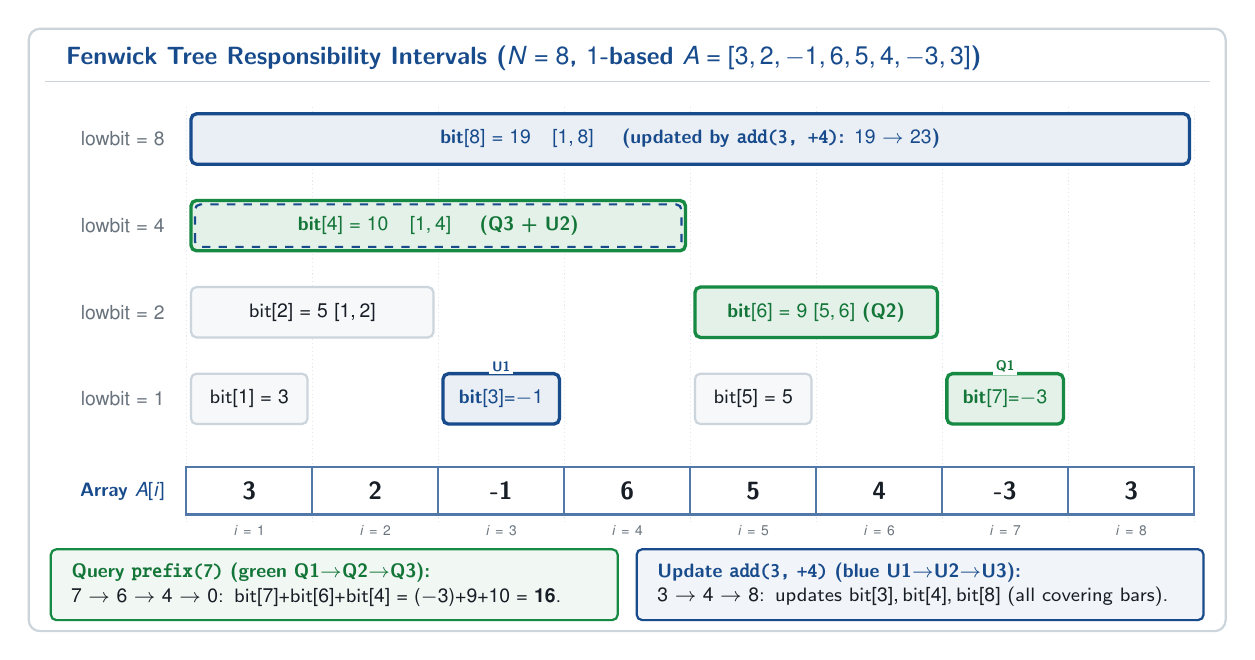
\begin{tikzpicture}[x=1cm, y=1cm]
    % Outer container frame: 0.0 to 15.2 cm
    \draw[codeframe, thick, rounded corners=4pt, fill=white] (0, 0) rectangle (15.2, 7.65);

    % Header strip
    \node[anchor=west, font=\small\bfseries, text=primaryblue] at (0.35, 7.28)
        {Fenwick Tree Responsibility Intervals ($N = 8$, $1$-based $A = [3, 2, -1, 6, 5, 4, -3, 3]$)};
    \draw[codeframe, thin] (0.2, 6.98) -- (15.0, 6.98);

    % Left axis labels for lowbit tiers (x = 0.2 .. 1.9)
    % 8 columns spanning x = 2.0 to 14.8 -> each column width = 1.60 cm
    % Column i center: 2.0 + (i - 0.5) * 1.60; column i spans [2.0 + (i-1)*1.60, 2.0 + i*1.60]
    \node[anchor=east, font=\scriptsize\bfseries, text=codegray] at (1.85, 6.25) {$\operatorname{lowbit}=8$};
    \node[anchor=east, font=\scriptsize\bfseries, text=codegray] at (1.85, 5.15) {$\operatorname{lowbit}=4$};
    \node[anchor=east, font=\scriptsize\bfseries, text=codegray] at (1.85, 4.05) {$\operatorname{lowbit}=2$};
    \node[anchor=east, font=\scriptsize\bfseries, text=codegray] at (1.85, 2.95) {$\operatorname{lowbit}=1$};
    \node[anchor=east, font=\scriptsize\bfseries, text=primaryblue] at (1.85, 1.78) {Array $A[i]$};

    % Subtle vertical column guide lines
    \foreach \c in {0,1,...,8} {
        \draw[codeframe!55, densely dotted] ({2.0 + \c*1.60}, 1.38) -- ({2.0 + \c*1.60}, 6.68);
    }

    % Row 4: lowbit = 8 -> bit[8] covers [1,8] = 19 (touched by add(3,+4) -> blue border!)
    \draw[primaryblue, very thick, fill=primaryblue!9, rounded corners=2pt]
        (2.06, 5.93) rectangle (14.74, 6.57);
    \node[font=\scriptsize\bfseries, text=primaryblue] at (8.40, 6.25)
        {$\text{bit}[8] = 19 \quad [1, 8]$ \quad (updated by \texttt{add(3, +4)}: $19 \to 23$)};

    % Row 3: lowbit = 4 -> bit[4] covers [1,4] = 10 (BOTH query(7) AND add(3,+4)!)
    \draw[codegreen, very thick, fill=codegreen!12, rounded corners=2pt]
        (2.06, 4.83) rectangle (8.34, 5.47);
    \draw[primaryblue, thick, dashed, rounded corners=2pt]
        (2.11, 4.88) rectangle (8.29, 5.42);
    \node[font=\scriptsize\bfseries, text=codegreen!85!black] at (5.20, 5.15)
        {$\text{bit}[4] = 10 \quad [1, 4]$ \quad (Q3 + U2)};

    % Row 2: lowbit = 2 -> bit[2] covers [1,2] = 5; bit[6] covers [5,6] = 9 (query(7)!)
    \draw[codeframe, thick, fill=codebg, rounded corners=2pt]
        (2.06, 3.73) rectangle (5.14, 4.37);
    \node[font=\scriptsize, text=codeink] at (3.60, 4.05) {$\text{bit}[2] = 5\;[1,2]$};

    \draw[codegreen, very thick, fill=codegreen!12, rounded corners=2pt]
        (8.46, 3.73) rectangle (11.54, 4.37);
    \node[font=\scriptsize\bfseries, text=codegreen!85!black] at (10.00, 4.05) {$\text{bit}[6] = 9\;[5,6]$ (Q2)};

    % Row 1: lowbit = 1 -> bit[1]=3, bit[3]=-1 (U1), bit[5]=5, bit[7]=-3 (Q1)
    \draw[codeframe, thick, fill=codebg, rounded corners=2pt]
        (2.06, 2.63) rectangle (3.54, 3.27);
    \node[font=\scriptsize, text=codeink] at (2.80, 2.95) {$\text{bit}[1]=3$};

    \draw[primaryblue, very thick, fill=primaryblue!9, rounded corners=2pt]
        (5.26, 2.63) rectangle (6.74, 3.27);
    \node[font=\scriptsize\bfseries, text=primaryblue] at (6.00, 2.95) {$\text{bit}[3]{=}{-}1$};
    \node[font=\tiny\bfseries, text=primaryblue, fill=white, inner sep=1pt] at (6.00, 3.36) {U1};

    \draw[codeframe, thick, fill=codebg, rounded corners=2pt]
        (8.46, 2.63) rectangle (9.94, 3.27);
    \node[font=\scriptsize, text=codeink] at (9.20, 2.95) {$\text{bit}[5]=5$};

    \draw[codegreen, very thick, fill=codegreen!12, rounded corners=2pt]
        (11.66, 2.63) rectangle (13.14, 3.27);
    \node[font=\scriptsize\bfseries, text=codegreen!85!black] at (12.40, 2.95) {$\text{bit}[7]{=}{-}3$};
    \node[font=\tiny\bfseries, text=codegreen!85!black, fill=white, inner sep=1pt] at (12.40, 3.36) {Q1};

    % Bottom base array A[1..8]
    \foreach \idx/\val in {1/3, 2/2, 3/-1, 4/6, 5/5, 6/4, 7/-3, 8/3} {
        \pgfmathsetmacro{\xL}{2.0 + (\idx - 1)*1.60}
        \pgfmathsetmacro{\xC}{2.0 + (\idx - 0.5)*1.60}
        \draw[primaryblue!75, thick, fill=white] (\xL, 1.48) rectangle ({\xL + 1.60}, 2.08);
        \node[font=\small\bfseries, text=codeink] at (\xC, 1.78) {\val};
        \node[font=\tiny\color{codegray}] at (\xC, 1.28) {$i=\idx$};
    }

    % Bottom Legend / Dual Trace Summary Strip (y = 0.14 .. 1.04)
    \draw[codegreen, thick, fill=codegreen!6, rounded corners=2pt] (0.28, 0.14) rectangle (7.48, 1.04);
    \node[anchor=west, font=\scriptsize, text=codeink, text width=6.95cm] at (0.42, 0.59) {
        \textbf{\color{codegreen!85!black}Query \texttt{prefix(7)} (green Q1$\to$Q2$\to$Q3):}\\[1pt]
        $7 \to 6 \to 4 \to 0$: $\text{bit}[7]{+}\text{bit}[6]{+}\text{bit}[4] = (-3){+}9{+}10 = \mathbf{16}$.
    };

    \draw[primaryblue, thick, fill=primaryblue!6, rounded corners=2pt] (7.72, 0.14) rectangle (14.92, 1.04);
    \node[anchor=west, font=\scriptsize, text=codeink, text width=6.95cm] at (7.86, 0.59) {
        \textbf{\color{primaryblue}Update \texttt{add(3, +4)} (blue U1$\to$U2$\to$U3):}\\[1pt]
        $3 \to 4 \to 8$: updates $\text{bit}[3], \text{bit}[4], \text{bit}[8]$ (all covering bars).
    };
\end{tikzpicture}
\caption{Fenwick Tree responsibility bars for $N = 8$. Each bucket $\text{bit}[i]$ covers $[i - \operatorname{lowbit}(i) + 1,\, i]$. Stripping lowbits (\texttt{i -= i \& -i}) partitions $[1, 7]$ into three disjoint green bars; adding lowbits (\texttt{i += i \& -i}) climbs every bar covering index $3$.}
\label{fig:fenwick_intervals}
\end{figure}

\begin{watchoutbox}[Watch Out --- Zero-Based Indexing Causes an Infinite Loop!]
Never index a Fenwick Tree from $0$! In two's complement arithmetic, $0 \mathbin{\&} (-0) = 0$. Therefore:
\begin{itemize}[itemsep=2pt, topsep=2pt]
    \item \texttt{for (int i = 0; i <= n; i += i \& -i)} spins forever at \texttt{i = 0}.
    \item \texttt{while (i >= 0) \{ sum += bit[i]; i -= i \& -i; \}} spins forever at \texttt{i = 0}.
\end{itemize}
Always keep the internal \texttt{bit} array \textbf{1-based} (\texttt{bit[1..N]} with unused \texttt{bit[0] = 0}). If your caller uses 0-based indices, convert immediately at the public API boundary via \texttt{++idx}.
\end{watchoutbox}

\begin{tryitbox}{Trace}{Build, Update, and Query a Fenwick Tree by Hand}{ex2}
Given the $1$-based array $A = [4, 1, 5, -2, 3, 7, 0, 2]$ ($N = 8$):
\begin{enumerate}[itemsep=2pt, topsep=2pt]
    \item Compute all $8$ entries of $\text{bit}[1..8]$.
    \item Trace \texttt{add(3, +5)}: list every index updated and its new value.
    \item After that update, trace \texttt{range\_sum(2, 7)} via $\operatorname{prefix}(7) - \operatorname{prefix}(1)$ and verify the final answer.
\end{enumerate}
\end{tryitbox}

\subsection{Linear \texorpdfstring{$O(N)$}{O(N)} Build and Range-Add via Difference BIT}

\textbf{Building in $O(N)$ instead of $O(N \log N)$.} Calling \texttt{add(i, A[i])} for each $i = 1 \dots N$ works in $O(N \log N)$, but we can build the exact same BIT in strict $O(N)$ time. Copy $A[1..N]$ into $\text{bit}[1..N]$, then sweep $i = 1 \dots N$ once:
$$\text{let } j = i + (i \mathbin{\&} (-i)); \quad \text{if } j \le N, \quad \text{bit}[j] \mathrel{+}= \text{bit}[i].$$
Why is this exact? When the loop reaches index $i$, every smaller bucket whose immediate parent is $i$ has already added its completed sum into $\text{bit}[i]$. Pushing $\text{bit}[i]$ once to its \emph{immediate} parent $j = i + \operatorname{lowbit}(i)$ propagates $A[i]$ cleanly up the entire ancestor chain without redundant touches.

\textbf{Range-Add + Point-Query (Difference BIT).} Recall Difference Arrays from Module~04: define $D[1] = A[1]$ and $D[i] = A[i] - A[i - 1]$ for $i \ge 2$, so $A[k] = \sum_{i=1}^{k} D[i]$. Storing $D$ inside a single Fenwick Tree lets you add $\delta$ to every element in $[l, r]$ in $O(\log N)$ via just two point updates:
\begin{itemize}[itemsep=2pt, topsep=2pt]
    \item \texttt{bit.add(l, +delta)}
    \item \texttt{if (r + 1 <= N) bit.add(r + 1, -delta)}
\end{itemize}
Then \texttt{point\_query(k)} is simply $\operatorname{prefix}_D(k)$ in $O(\log N)$!

\textbf{Range-Add + Range-Sum (Two-BIT Identity).} What if you need \emph{both} range-add and range-sum without writing a Lazy Segment Tree? Sum the difference identity $A[k] = \sum_{i=1}^{k} D[i]$ over $k = 1 \dots p$ and swap the order of summation:
\begin{formulabox}[Two-BIT Range-Add + Range-Sum Formula]
$$\sum_{k=1}^{p} A[k] = \sum_{k=1}^{p} \sum_{i=1}^{k} D[i] = \sum_{i=1}^{p} (p - i + 1)\, D[i] = p \sum_{i=1}^{p} D[i] - \sum_{i=1}^{p} (i - 1)\, D[i]$$
\textbf{Read this as:} Maintain two Fenwick Trees: $B_1$ stores $D[i]$ and $B_2$ stores $(i - 1)\,D[i]$.
\begin{itemize}[itemsep=2pt, topsep=2pt]
    \item \textbf{Range add $+\delta$ on $[l, r]$:} update $B_1$ with $(l, +\delta)$ and $(r+1, -\delta)$; update $B_2$ with $(l, +\delta(l-1))$ and $(r+1, -\delta r)$ (whenever $r + 1 \le N$).
    \item \textbf{Prefix sum $[1, p]$:} return $p \cdot \operatorname{prefix}_{B_1}(p) - \operatorname{prefix}_{B_2}(p)$.
\end{itemize}
\end{formulabox}

\examplebeat Start with six zeros $A = [0, 0, 0, 0, 0, 0]$. Apply \texttt{range\_add(2, 5, +3)} then \texttt{range\_add(4, 6, +2)}, producing logical array $A = [0, 3, 3, 5, 5, 2]$. At $p = 5$: $D[1..5] = [0, 3, 0, 2, 0]$, so $\operatorname{prefix}_{B_1}(5) = 5$ and $\operatorname{prefix}_{B_2}(5) = 1 \cdot 3 + 3 \cdot 2 = 9$. The formula gives $5 \cdot 5 - 9 = 16$, matching $0 + 3 + 3 + 5 + 5 = 16$!

\begin{tryitbox}{Debug}{Spot Two Bugs in a Broken Fenwick Snippet}{ex3}
A programmer wrote the following $0$-based Fenwick helper for array size $n$:
\begin{quote}\ttfamily\small
void add(int i, long long d) \{ for (; i < n; i += i \& -i) bit[i] += d; \}\\
long long range\_sum(int l, int r) \{ return prefix(r) - prefix(l); \}
\end{quote}
Identify \textbf{both} bugs and give the smallest concrete input that triggers each failure.
\end{tryitbox}

\subsection{Binary Lifting on a Fenwick Tree (\texorpdfstring{$O(\log N)$}{O(log N)} Order Statistics)}

\painbeat Suppose $\text{bit}[1..N]$ stores non-negative frequencies of values $1 \dots N$ and you want the $K$-th smallest element --- i.e., the smallest index $p$ such that $\operatorname{prefix}(p) \ge K$. Running binary search on $p \in [1, N]$ and calling $\operatorname{prefix}(\text{mid})$ inside each step takes $O(\log N) \times O(\log N) = O(\log^2 N)$.

\ahabeat Every Fenwick bucket at an aligned power-of-two jump \texttt{pos + step} \emph{already} stores the exact disjoint sum of the block $(\text{pos},\; \text{pos} + \text{step}]$! Start with $\text{pos} = 0$ and $\text{step} = 2^{\lfloor \log_2 N \rfloor}$ (computed in C++20 via \texttt{std::bit\_floor(n)}). At each bit from high to low:
\begin{itemize}[itemsep=2pt, topsep=2pt]
    \item Check if $\text{pos} + \text{step} \le N$ \textbf{and} $\text{bit}[\text{pos} + \text{step}] < K$.
    \item If true, this entire block still leaves us strictly below $K$: commit the jump $\text{pos} \mathrel{+}= \text{step}$ and subtract $K \mathrel{-}= \text{bit}[\text{pos}]$.
    \item Halve $\text{step} \gg= 1$ and repeat until $\text{step} = 0$.
\end{itemize}
\invariantbeat{BIT Binary Lifting} At every step, $\text{pos}$ is the largest committed prefix whose sum is strictly less than the original target $K_{\text{orig}}$, and $K$ equals $K_{\text{orig}} - \operatorname{prefix}(\text{pos}) > 0$. When the loop ends, $\text{pos} + 1$ is the exact first index with $\operatorname{prefix}(p) \ge K_{\text{orig}}$ (or $N + 1$ if total sum $< K_{\text{orig}}$), in a single $O(\log N)$ pass!

\begin{watchoutbox}[Watch Out --- Non-Negative Weights Are Mandatory for Binary Lifting]
BIT binary lifting assumes $\operatorname{prefix}(p)$ is \textbf{monotonically non-decreasing} ($A[i] \ge 0$ for all $i$). Suppose $A = [5, -4, 3, 2]$ ($1$-based), whose prefix sums are $[5, 1, 4, 6]$ and BIT array is $\text{bit} = [5, 1, 3, 6]$. Seeking the first prefix $\ge 4$ (true answer: index $1$, where $\operatorname{prefix}(1) = 5$):
\begin{itemize}[itemsep=1pt, topsep=1pt]
    \item $\text{step} = 4$: $\text{bit}[4] = 6 \not< 4 \to$ skip.
    \item $\text{step} = 2$: $\text{bit}[2] = 1 < 4 \to$ \textbf{jumps to $\text{pos} = 2$}, $K \leftarrow 3$ (leaps straight over index $1$!).
    \item $\text{step} = 1$: $\text{bit}[3] = 3 \not< 3 \to$ skip, returning wrong answer $\text{pos} + 1 = 3$.
\end{itemize}
\end{watchoutbox}

\begin{tryitbox}{Trace}{Binary Lifting on a Frequency BIT}{ex4}
Let $A = [2, 0, 3, 1, 0, 2, 1, 1]$ ($1$-based, $N = 8$), whose BIT array is $\text{bit}[1..8] = [2, 2, 3, 6, 0, 2, 1, 10]$. Trace \texttt{lower\_bound(K = 7)} for $\text{step} = 8, 4, 2, 1$, recording $(\text{step},\; \text{pos} + \text{step},\; \text{bit}[\text{pos}+\text{step}],\; K,\; \text{TAKE/SKIP})$ at each iteration and verifying the final index $\text{pos} + 1$.
\end{tryitbox}

% ============================================================================
\section{Segment Trees: Universal Monoid Range Queries}
% ============================================================================

When your operation has no inverse ($\min, \max, \gcd$, maximum subarray sum, matrix product), a Fenwick Tree cannot subtract prefixes. A \textbf{Segment Tree} solves every associative monoid by storing a complete binary tree of interval summaries directly.

\begin{notationbox}[Symbols Used in Section 3]
$(S, \oplus, e)$ & Associative monoid: binary merge $\oplus$ with identity $e$ ($e \oplus x = x \oplus e = x$). & $(\mathbb{Z}, \min, +\infty)$ \\
$v$ & $1$-based heap index of a Segment Tree node (children $2v$ and $2v + 1$). & Root $v = 1$ \\
$[tl, tr]$ & Inclusive array segment owned by node $v$ in a recursive tree. & $[0, N-1]$ \\
$[l, r]$ / $[l, r)$ & Requested query interval (inclusive in recursive; half-open in iterative). & $[1, 4]$ or $[1, 5)$ \\
$\text{res}_L, \text{res}_R$ & Left and right accumulators preserving order for non-commutative $\oplus$. & Init to $e$ \\
\end{notationbox}

\subsection{Recursive Segment Tree (Top-Down, \texorpdfstring{$4N$}{4N} Layout)}

\painbeat How do we answer $\min(A[l..r])$ after arbitrary point assignments \texttt{A[pos] = val} without scanning $[l, r]$?

\ahabeat Represent the full array $[0, N - 1]$ at root $v = 1$. Recursively split any interval $[tl, tr]$ with $tl < tr$ at midpoint $tm = \lfloor (tl + tr) / 2 \rfloor$:
\begin{itemize}[itemsep=2pt, topsep=2pt]
    \item Left child $2v$ owns $[tl, tm]$; right child $2v + 1$ owns $[tm + 1, tr]$.
    \item Each internal node stores $\text{tree}[v] = \text{tree}[2v] \oplus \text{tree}[2v + 1]$.
\end{itemize}

When querying $[l, r]$ at node $v$ owning $[tl, tr]$, exactly three cases exist:
\begin{enumerate}[itemsep=2pt, topsep=2pt]
    \item \textbf{Disjoint ($r < tl$ or $tr < l$):} Return the identity element $e$ immediately (prune!).
    \item \textbf{Completely Covered ($l \le tl$ and $tr \le r$):} Return $\text{tree}[v]$ directly without recursing!
    \item \textbf{Partial Overlap:} Recurse into $2v$ and $2v + 1$ and return $\text{left\_res} \oplus \text{right\_res}$.
\end{enumerate}

\examplebeat Build a Range-Minimum Segment Tree over $A = [5, 2, 7, 1, 8, 3]$ ($N = 6$) and trace \texttt{query(1, 4)} (Figure~\ref{fig:segtree_recursive}). The query stops immediately at three green full-cover nodes --- $v = 9$ ($[1, 1] \to 2$), $v = 5$ ($[2, 2] \to 7$), and $v = 6$ ($[3, 4] \to 1$) --- never even visiting leaves $v = 12$ or $v = 13$, and returns $\min(2, 7, 1) = 1$.

\begin{figure}[htbp]
\centering
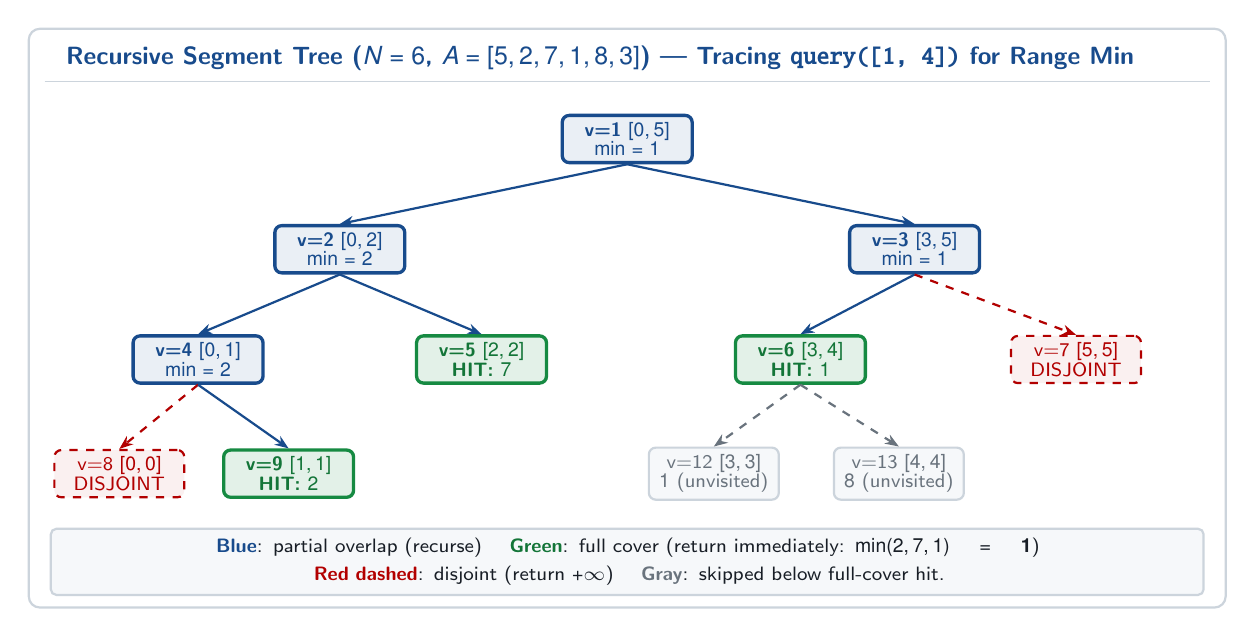
\begin{tikzpicture}[x=1cm, y=1cm,
    stnode/.style={draw=codeframe, fill=codebg, thick, rounded corners=2.5pt, align=center, inner sep=2.5pt, font=\scriptsize, minimum width=1.65cm},
    stpart/.style={draw=primaryblue, fill=primaryblue!9, very thick, rounded corners=2.5pt, align=center, inner sep=2.5pt, font=\scriptsize, text=primaryblue, minimum width=1.65cm},
    sthit/.style={draw=codegreen, fill=codegreen!12, very thick, rounded corners=2.5pt, align=center, inner sep=2.5pt, font=\scriptsize\bfseries, text=codegreen!85!black, minimum width=1.65cm},
    stprune/.style={draw=red!70!black, fill=red!70!black!6, thick, dashed, rounded corners=2.5pt, align=center, inner sep=2.5pt, font=\scriptsize, text=red!70!black, minimum width=1.65cm}
]
    % Frame 0.0 to 15.2 cm
    \draw[codeframe, thick, rounded corners=4pt, fill=white] (0, 0) rectangle (15.2, 7.35);
    \node[anchor=west, font=\small\bfseries, text=primaryblue] at (0.35, 6.98)
        {Recursive Segment Tree ($N = 6$, $A = [5, 2, 7, 1, 8, 3]$) --- Tracing \texttt{query([1, 4])} for Range Min};
    \draw[codeframe, thin] (0.2, 6.68) -- (15.0, 6.68);

    % Level 0 (y = 5.95)
    \node[stpart] (v1) at (7.60, 5.95) {\textbf{v=1} $[0,5]$\\[-1pt]$\min = 1$};

    % Level 1 (y = 4.55)
    \node[stpart] (v2) at (3.95, 4.55) {\textbf{v=2} $[0,2]$\\[-1pt]$\min = 2$};
    \node[stpart] (v3) at (11.25, 4.55) {\textbf{v=3} $[3,5]$\\[-1pt]$\min = 1$};

    % Level 2 (y = 3.15)
    \node[stpart] (v4) at (2.15, 3.15) {\textbf{v=4} $[0,1]$\\[-1pt]$\min = 2$};
    \node[sthit]  (v5) at (5.75, 3.15) {v=5 $[2,2]$\\[-1pt]HIT: $7$};
    \node[sthit]  (v6) at (9.80, 3.15) {v=6 $[3,4]$\\[-1pt]HIT: $1$};
    \node[stprune] (v7) at (13.30, 3.15) {v=7 $[5,5]$\\[-1pt]DISJOINT};

    % Level 3 (y = 1.70)
    \node[stprune] (v8) at (1.15, 1.70) {v=8 $[0,0]$\\[-1pt]DISJOINT};
    \node[sthit]   (v9) at (3.30, 1.70) {v=9 $[1,1]$\\[-1pt]HIT: $2$};
    \node[stnode]  (v12) at (8.70, 1.70) {\color{codegray}v=12 $[3,3]$\\[-1pt]\color{codegray}$1$ (unvisited)};
    \node[stnode]  (v13) at (11.05, 1.70) {\color{codegray}v=13 $[4,4]$\\[-1pt]\color{codegray}$8$ (unvisited)};

    % Edges
    \draw[lmarrow] (v1.south) -- (v2.north);
    \draw[lmarrow] (v1.south) -- (v3.north);
    \draw[lmarrow] (v2.south) -- (v4.north);
    \draw[lmarrow] (v2.south) -- (v5.north);
    \draw[lmarrow] (v3.south) -- (v6.north);
    \draw[lmprunedarrow] (v3.south) -- (v7.north);
    \draw[lmprunedarrow] (v4.south) -- (v8.north);
    \draw[lmarrow] (v4.south) -- (v9.north);
    \draw[lmmuted, dashed] (v6.south) -- (v12.north);
    \draw[lmmuted, dashed] (v6.south) -- (v13.north);

    % Legend / Summary strip (y = 0.16 .. 1.00)
    \draw[codeframe, thick, fill=codebg, rounded corners=2pt] (0.28, 0.16) rectangle (14.92, 1.00);
    \node[anchor=center, font=\scriptsize, text=codeink, text width=14.35cm, align=center] at (7.60, 0.58) {
        \textbf{\color{primaryblue}Blue}: partial overlap (recurse) \quad
        \textbf{\color{codegreen!85!black}Green}: full cover (return immediately: $\min(2, 7, 1) = \mathbf{1}$)\\[2pt]
        \textbf{\color{red!70!black}Red dashed}: disjoint (return $+\infty$) \quad
        \textbf{\color{codegray}Gray}: skipped below full-cover hit.
    };
\end{tikzpicture}
\caption{Recursive Segment Tree on $A = [5, 2, 7, 1, 8, 3]$ ($N = 6$). Notice that the deepest leaf reaches heap index $v = 13 > 2N = 12$, demonstrating why recursive trees allocate $4N$ storage.}
\label{fig:segtree_recursive}
\end{figure}

\textbf{Why does a query take $O(\log N)$ time?} At any single tree depth, at most \emph{two} nodes can partially overlap $[l, r]$: the unique node straddling left boundary $l$, and the unique node straddling right boundary $r$. Every node strictly between them is fully covered (stops immediately), and every node outside is disjoint (stops immediately). Because at most $2$ nodes per level split into $2$ children each, a query visits \textbf{at most $4 \lceil \log_2 N \rceil$} nodes in total!

\textbf{Why allocate $4N$ memory (never $2N$)?} Every split halves the segment length, so all leaves sit at depth $d \le \lceil \log_2 N \rceil$. Let $P = 2^{\lceil \log_2 N \rceil}$ be the smallest power of $2$ with $P \ge N$. Then $P \le 2N - 2$ for every $N \ge 2$ (and $P = 1$ for $N = 1$), so the maximum $1$-based heap index ever reached is:
$$v_{\max} \le 2^{\lceil \log_2 N \rceil + 1} - 1 = 2P - 1 < 4N.$$
As Figure~\ref{fig:segtree_recursive} already proved for $N = 6$, the deepest leaf sits at $v = 13 > 2N = 12$, so a $2N$-sized recursive array causes an out-of-bounds buffer overflow!

\begin{tryitbox}{Derive}{Exact Maximum Heap Index in a Recursive Segment Tree}{ex5}
Using the standard split $tm = \lfloor (tl + tr) / 2 \rfloor$ with root $v = 1$ covering $[0, N - 1]$:
\begin{enumerate}[itemsep=2pt, topsep=2pt]
    \item Find the exact largest node index $v_{\max}$ reached when $N = 5$ and when $N = 10$.
    \item Explain why $N = 5$ stays under $2N = 10$, whereas $N = 6$ ($v_{\max} = 13$) and $N = 10$ exceed $2N$.
\end{enumerate}
\end{tryitbox}

\subsection{Iterative Bottom-Up Segment Tree (\texorpdfstring{$2N$}{2N} Layout, Half-Open \texorpdfstring{$[l, r)$}{[l, r)})}

\painbeat Recursive Segment Trees allocate $4N$ memory and pay recursive call-frame overhead on every node visit. For point updates and range queries (without lazy propagation), can we cut memory in half and eliminate recursion completely?

\ahabeat Place all $N$ leaves contiguously in the second half of a $2N$-element array: leaf $i$ lives at $\text{tree}[N + i]$ ($0 \le i < N$). Then fill internal nodes bottom-up from $i = N - 1$ down to $1$:
$$\text{tree}[i] = \text{tree}[2i] \oplus \text{tree}[2i + 1].$$
Notice that even when $N$ is \emph{not} a power of $2$, every internal node still represents a contiguous (or wrap-split, still disjoint!) partition of leaves, and every leaf's ancestors are reached simply by dividing by $2$ (\texttt{pos >>= 1})!

To answer a \textbf{half-open} query $[l, r)$ ($0 \le l \le r \le N$): shift both endpoints to the leaf layer ($l \mathrel{+}= N$, $r \mathrel{+}= N$). While $l < r$:
\begin{itemize}[itemsep=2pt, topsep=2pt]
    \item If $l$ is \textbf{odd} (\texttt{l \& 1}), node $l$ is a right child whose left sibling lies \emph{outside} $[l, r)$. We cannot climb to its parent, so we consume $\text{tree}[l]$ into $\text{res}_L$ and step right (\texttt{l++}).
    \item If $r$ is \textbf{odd} (\texttt{r \& 1}), then $r - 1$ is an \emph{even} left child inside $[l, r)$ whose right sibling $r$ lies outside. Decrement \texttt{--r} and prepend $\text{tree}[r]$ onto $\text{res}_R$.
    \item Both $l$ and $r$ are now even; climb one level via \texttt{l >>= 1; r >>= 1;}.
\end{itemize}

\begin{figure}[htbp]
\centering
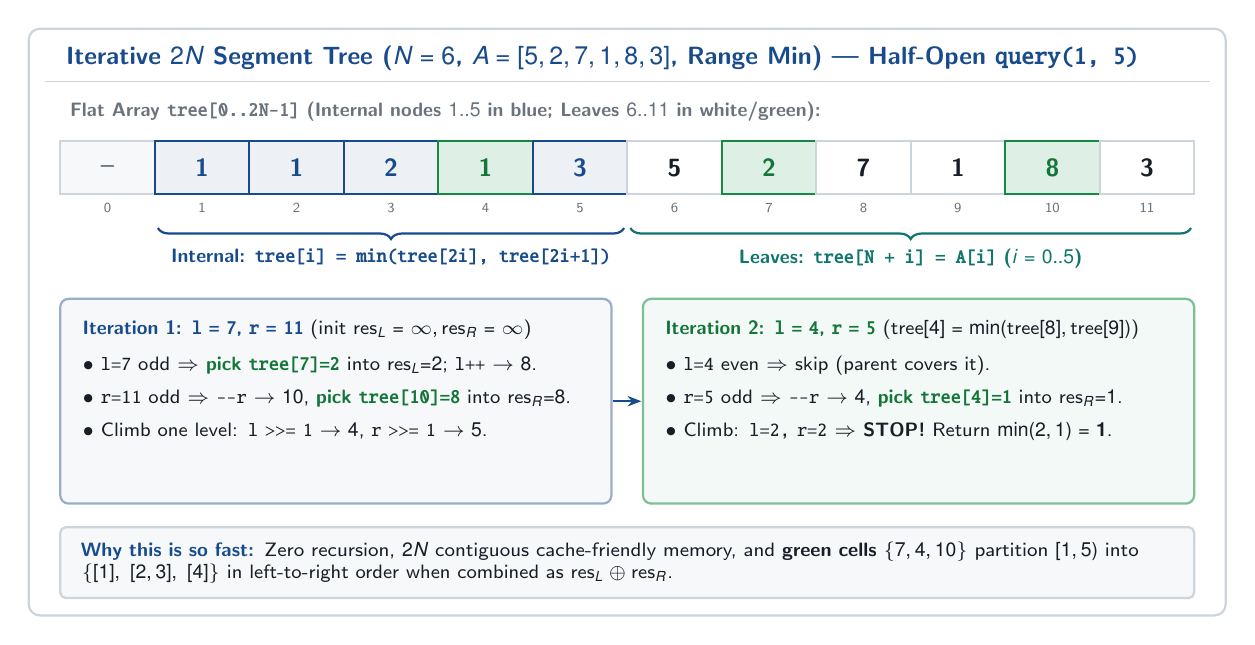
\begin{tikzpicture}[x=1cm, y=1cm]
    % Outer container frame 0..15.2 cm (expanded height 7.45 cm for generous card clearance)
    \draw[codeframe, thick, rounded corners=4pt, fill=white] (0, 0) rectangle (15.2, 7.45);
    \node[anchor=west, font=\small\bfseries, text=primaryblue] at (0.35, 7.08)
        {Iterative $2N$ Segment Tree ($N = 6$, $A = [5, 2, 7, 1, 8, 3]$, Range Min) --- Half-Open \texttt{query(1, 5)}};
    \draw[codeframe, thin] (0.2, 6.78) -- (15.0, 6.78);

    % Flat 2N array cells: indices 0..11 across x = 0.40 .. 14.80 (12 cells * 1.20 cm)
    \node[anchor=west, font=\scriptsize\bfseries, text=codegray] at (0.40, 6.40) {Flat Array \texttt{tree[0..2N-1]} (Internal nodes $1..5$ in blue; Leaves $6..11$ in white/green):};

    \foreach \idx/\val/\fillc/\bordc/\txtc in {
        0/{--}/codebg/codeframe/codegray,
        1/1/primaryblue!8/primaryblue/primaryblue,
        2/1/primaryblue!8/primaryblue/primaryblue,
        3/2/primaryblue!8/primaryblue/primaryblue,
        4/1/codegreen!14/codegreen/codegreen!85!black,
        5/3/primaryblue!8/primaryblue/primaryblue,
        6/5/white/codeframe/codeink,
        7/2/codegreen!14/codegreen/codegreen!85!black,
        8/7/white/codeframe/codeink,
        9/1/white/codeframe/codeink,
        10/8/codegreen!14/codegreen/codegreen!85!black,
        11/3/white/codeframe/codeink%
    } {
        \pgfmathsetmacro{\xL}{0.40 + \idx*1.20}
        \pgfmathsetmacro{\xC}{\xL + 0.60}
        \draw[\bordc, thick, fill=\fillc] (\xL, 5.35) rectangle ({\xL + 1.20}, 6.02);
        \node[font=\small\bfseries, text=\txtc] at (\xC, 5.69) {\val};
        \node[font=\tiny\color{codegray}] at (\xC, 5.17) {\idx};
    }

    % Braces below internal vs leaf halves
    \draw[decorate, decoration={brace, amplitude=4pt, mirror}, primaryblue, thick]
        (1.64, 4.92) -- (7.56, 4.92) node[midway, below=4pt, font=\scriptsize\bfseries, text=primaryblue] {Internal: \texttt{tree[i] = min(tree[2i], tree[2i+1])}};
    \draw[decorate, decoration={brace, amplitude=4pt, mirror}, accentteal, thick]
        (7.64, 4.92) -- (14.76, 4.92) node[midway, below=4pt, font=\scriptsize\bfseries, text=accentteal] {Leaves: \texttt{tree[N + i] = A[i]} ($i = 0..5$)};

    % Two step cards tracing query(1, 5) -> l = 1+6=7, r = 5+6=11 (tall 2.55 cm cards!)
    \draw[primaryblue!45, thick, fill=primaryblue!4, rounded corners=3pt] (0.40, 1.42) rectangle (7.40, 4.02);
    \node[anchor=north west, font=\scriptsize, text=codeink, text width=6.68cm] at (0.56, 3.88) {
        \textbf{\color{primaryblue}Iteration 1: \texttt{l = 7}, \texttt{r = 11}} (init $\text{res}_L = \infty, \text{res}_R = \infty$)\\[5pt]
        $\bullet$ \texttt{l=7} odd $\Rightarrow$ \textbf{\color{codegreen!85!black}pick \texttt{tree[7]=2}} into $\text{res}_L{=}2$; \texttt{l++} $\to 8$.\\[4pt]
        $\bullet$ \texttt{r=11} odd $\Rightarrow$ \texttt{--r} $\to 10$, \textbf{\color{codegreen!85!black}pick \texttt{tree[10]=8}} into $\text{res}_R{=}8$.\\[4pt]
        $\bullet$ Climb one level: \texttt{l >>= 1} $\to 4$, \texttt{r >>= 1} $\to 5$.
    };

    \draw[codegreen!55, thick, fill=codegreen!5, rounded corners=3pt] (7.80, 1.42) rectangle (14.80, 4.02);
    \node[anchor=north west, font=\scriptsize, text=codeink, text width=6.68cm] at (7.96, 3.88) {
        \textbf{\color{codegreen!85!black}Iteration 2: \texttt{l = 4}, \texttt{r = 5}} ($\text{tree}[4] = \min(\text{tree}[8], \text{tree}[9])$)\\[5pt]
        $\bullet$ \texttt{l=4} even $\Rightarrow$ skip (parent covers it).\\[4pt]
        $\bullet$ \texttt{r=5} odd $\Rightarrow$ \texttt{--r} $\to 4$, \textbf{\color{codegreen!85!black}pick \texttt{tree[4]=1}} into $\text{res}_R{=}1$.\\[4pt]
        $\bullet$ Climb: \texttt{l=2, r=2} $\Rightarrow$ \textbf{STOP!} Return $\min(2, 1) = \mathbf{1}$.
    };

    % Arrow between Iteration 1 and Iteration 2
    \draw[lmarrow] (7.42, 2.72) -- (7.78, 2.72);

    % Bottom takeaway bar (y = 0.22 .. 1.12)
    \draw[codeframe, thick, fill=codebg, rounded corners=2pt] (0.40, 0.22) rectangle (14.80, 1.12);
    \node[anchor=west, font=\scriptsize, text=codeink, text width=14.1cm] at (0.55, 0.67) {
        \textbf{\color{primaryblue}Why this is so fast:} Zero recursion, $2N$ contiguous cache-friendly memory, and \textbf{green cells} $\{7, 4, 10\}$ partition $[1, 5)$ into $\{[1],\; [2, 3],\; [4]\}$ in left-to-right order when combined as $\text{res}_L \oplus \text{res}_R$.
    };
\end{tikzpicture}
\caption{Iterative bottom-up $2N$ Segment Tree on $N = 6$. Shifting $l, r$ by $+N$ and peeling odd boundaries inward answers any half-open query $[l, r)$ in a tight bit-shift loop.}
\label{fig:segtree_iterative}
\end{figure}

\begin{watchoutbox}[Watch Out --- Non-Commutative Monoids Require Two Accumulators!]
If $\oplus$ is \textbf{not commutative} (e.g., matrix multiplication, string concatenation, or maximum subarray sum), folding both boundaries into a single accumulator \texttt{res = op(res, tree[...])} scrambles the left-to-right order!

\examplebeat Concatenate $S = [\text{``a''}, \text{``b''}, \text{``c''}, \text{``d''}, \text{``e''}, \text{``f''}]$ on $[1, 5)$ (true answer: \texttt{"bcde"}). On iteration 1, $l=7$ yields \texttt{"b"} and $r=10$ yields \texttt{"e"}; on iteration 2, $r=4$ yields \texttt{"cd"}.
\begin{itemize}[itemsep=1pt, topsep=1pt]
    \item \textbf{Buggy single accumulator:} appends \texttt{"b"} $\to$ \texttt{"e"} $\to$ \texttt{"cd"} $=$ \texttt{"becd"} (WRONG!).
    \item \textbf{Two accumulators:} $\text{res}_L = \text{res}_L \oplus \text{tree}[l\text{++}]$ builds \texttt{"b"}, while $\text{res}_R = \text{tree}[\text{--}r] \oplus \text{res}_R$ builds $\text{``cd''} \oplus \text{``e''} = \text{``cde''}$; finally $\text{res}_L \oplus \text{res}_R = \text{``bcde''}$ (EXACT!).
\end{itemize}
\end{watchoutbox}

\begin{tryitbox}{Trace}{Iterative $2N$ Query on a Sum Segment Tree}{ex6}
Build an iterative $2N$ \textbf{Range Sum} Segment Tree on $A = [4, 9, 3, 6, 2, 8]$ ($N = 6$):
\begin{enumerate}[itemsep=2pt, topsep=2pt]
    \item List $\text{tree}[1..11]$.
    \item Trace half-open \texttt{query(1, 5)}, showing $(l, r, \text{res}_L, \text{res}_R)$ after each iteration of \texttt{while (l < r)}.
\end{enumerate}
\end{tryitbox}

\subsection{Custom Monoid Nodes: Maximum Subarray Sum in a Range}

Segment Trees shine brightest when a single scalar cannot merge two halves. Suppose you must support point updates and answer: \emph{``What is the maximum sum of a non-empty contiguous subarray inside $[l, r]$?''}

Knowing only the best subarray inside left half $L$ and right half $R$ is insufficient, because the winning subarray might \textbf{cross the midpoint} (a suffix of $L$ glued to a prefix of $R$). Augment each node with four integers: $(\text{total},\; \text{pref},\; \text{suff},\; \text{best})$:

\begin{formulabox}[Maximum Subarray Sum Monoid Merge ($L \oplus R$)]
$$\begin{aligned}
\text{total} &= L.\text{total} + R.\text{total}, & \text{pref} &= \max(L.\text{pref},\; L.\text{total} + R.\text{pref}), \\
\text{suff} &= \max(R.\text{suff},\; R.\text{total} + L.\text{suff}), & \text{best} &= \max(L.\text{best},\; R.\text{best},\; L.\text{suff} + R.\text{pref}).
\end{aligned}$$
\textbf{Read this as:} A single leaf $x$ is $(x, x, x, x)$. The crossing candidate is always the best suffix of $L$ plus the best prefix of $R$. Because $\text{pref}$ and $\text{suff}$ are order-sensitive, this monoid is \textbf{non-commutative} --- so an iterative tree \emph{must} use $\text{res}_L$ and $\text{res}_R$ (or use an \texttt{optional} / sentinel identity)!
\end{formulabox}

% ============================================================================
\section{Lazy Propagation: \texorpdfstring{$O(\log N)$}{O(log N)} Range Updates AND Queries}
% ============================================================================

\begin{notationbox}[Symbols Used in Section 4]
$\text{lazy}[v]$ & Pending deferred update (``IOU note'') owed to $v$'s strict children ($2v, 2v+1$). & \texttt{int64\_t} or \texttt{optional} \\
$\text{apply}(v, tl, tr, \delta)$ & Updates $\text{tree}[v]$ immediately and records $\delta$ into $\text{lazy}[v]$ if $tl < tr$. & $O(1)$ helper \\
$\text{push}(v, tl, tr)$ & Sends $\text{lazy}[v]$ down to children $2v, 2v+1$ via \texttt{apply}, then clears $\text{lazy}[v]$. & Called before descent \\
$\text{pull}(v)$ & Recomputes $\text{tree}[v] = \text{tree}[2v] \oplus \text{tree}[2v+1]$ after returning from children. & Post-order refresh \\
\end{notationbox}

\subsection{Deferred Updates: \texttt{apply}, \texttt{push}, and \texttt{pull}}

\painbeat Suppose you need to add $+\delta$ to every element in $[l, r]$ and also query range sums (or range minimums) on arbitrary intervals. Updating every leaf in $[l, r]$ one by one takes $O((r - l + 1) \log N) = O(N \log N)$ per update --- slower than a plain loop!

\ahabeat Treat a Segment Tree node like a busy manager. When a range update $[l, r]$ completely covers node $v$'s interval $[tl, tr]$:
\begin{enumerate}[itemsep=2pt, topsep=2pt]
    \item \textbf{Update \texttt{tree[v]} immediately} so node $v$'s own summary is $100\%$ up to date (for range-add + range-sum, add $\delta \cdot (tr - tl + 1)$; for range-add + range-min, add $\delta$).
    \item \textbf{Stash an IOU note in \texttt{lazy[v]}} (if $v$ is not a leaf, $tl < tr$) remembering that $v$'s children have not heard about $+\delta$ yet, and \textbf{stop recursing}!
    \item \textbf{Pay the IOU only on demand (\texttt{push}):} Whenever a later update or query must descend into $2v$ and $2v + 1$, call \texttt{push(v)} \emph{before} stepping down so both children receive the pending update and $\text{lazy}[v]$ resets to empty.
\end{enumerate}

\invariantbeat{Lazy Propagation} Before and after every top-level operation, $\text{tree}[v]$ ALWAYS equals the exact aggregate of $[tl, tr]$ incorporating all updates whose tags sit at or below $v$ (so $\text{tree}[v]$ already includes $\text{lazy}[v]$), while $\text{lazy}[v]$ represents pending updates not yet reflected in $v$'s strict descendants.

\examplebeat Figure~\ref{fig:lazy_propagation} traces $A = [2, 1, 4, 3, 5, 2]$ ($N = 6$, Range Add + Range Sum) across two operations: Stage~A runs \texttt{range\_add([0, 4], +3)} and halts at $v = 2$ ($[0, 2]$) and $v = 6$ ($[3, 4]$); Stage~B runs \texttt{query([2, 3])}, which triggers \texttt{push} on both tagged nodes right before reading leaves $v = 5$ ($7$) and $v = 12$ ($6$) to return $13$.

\begin{figure}[htbp]
\centering
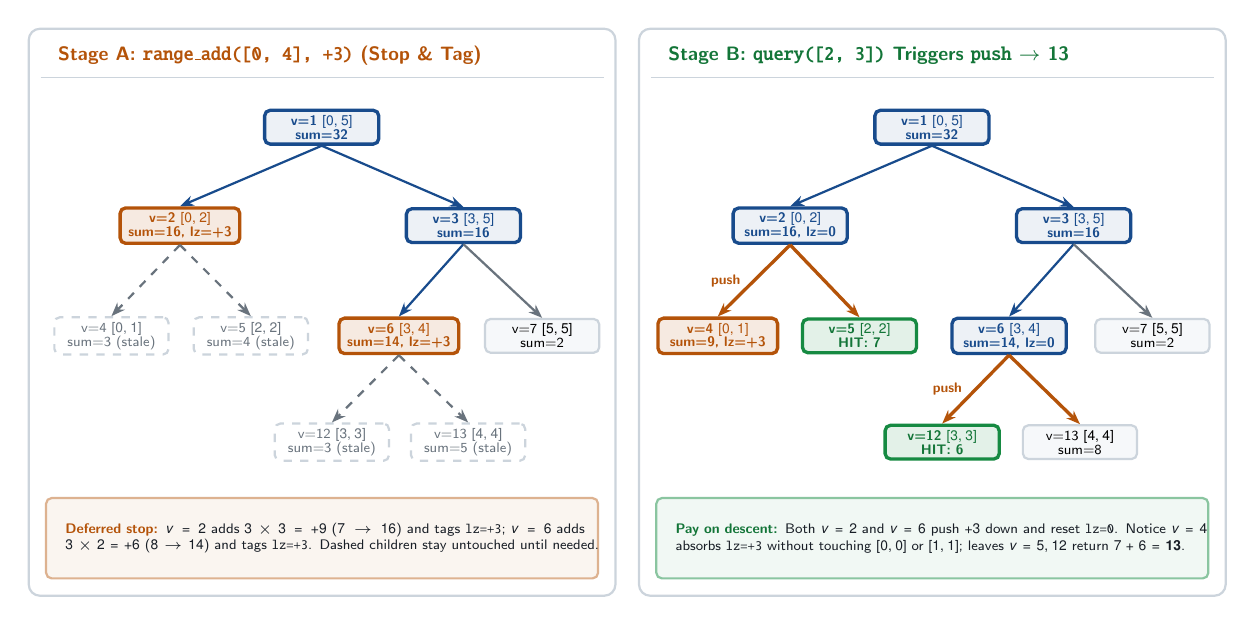
\begin{tikzpicture}[x=1cm, y=1cm,
    lnode/.style={draw=codeframe, fill=codebg, thick, rounded corners=2pt, align=center, inner sep=1.8pt, font=\tiny, minimum width=1.45cm},
    lstale/.style={draw=codeframe, fill=white, thick, dashed, rounded corners=2pt, align=center, inner sep=1.8pt, font=\tiny, text=codegray, minimum width=1.45cm},
    ltag/.style={draw=accentamber, fill=accentamber!12, very thick, rounded corners=2pt, align=center, inner sep=1.8pt, font=\tiny\bfseries, text=accentamber, minimum width=1.52cm},
    lhit/.style={draw=codegreen, fill=codegreen!12, very thick, rounded corners=2pt, align=center, inner sep=1.8pt, font=\tiny\bfseries, text=codegreen!85!black, minimum width=1.45cm},
    lpush/.style={draw=primaryblue, fill=primaryblue!8, very thick, rounded corners=2pt, align=center, inner sep=1.8pt, font=\tiny\bfseries, text=primaryblue, minimum width=1.45cm}
]
    % Left Panel: Stage A (x = 0.0 .. 7.45)
    \draw[codeframe, thick, rounded corners=4pt, fill=white] (0.0, 0.0) rectangle (7.45, 7.20);
    \node[anchor=west, font=\scriptsize\bfseries, text=accentamber] at (0.25, 6.86)
        {Stage A: \texttt{range\_add([0, 4], +3)} (Stop \& Tag)};
    \draw[codeframe, thin] (0.15, 6.58) -- (7.30, 6.58);

    % Left Tree coords (center 3.72)
    \node[lpush]  (a1) at (3.72, 5.95) {v=1 $[0,5]$\\[-1pt]sum=32};
    \node[ltag]   (a2) at (1.92, 4.70) {v=2 $[0,2]$\\[-1pt]sum=16, \textbf{lz=+3}};
    \node[lpush]  (a3) at (5.52, 4.70) {v=3 $[3,5]$\\[-1pt]sum=16};
    \node[lstale] (a4) at (1.05, 3.30) {v=4 $[0,1]$\\[-1pt]sum=3 (stale)};
    \node[lstale] (a5) at (2.82, 3.30) {v=5 $[2,2]$\\[-1pt]sum=4 (stale)};
    \node[ltag]   (a6) at (4.70, 3.30) {v=6 $[3,4]$\\[-1pt]sum=14, \textbf{lz=+3}};
    \node[lnode]  (a7) at (6.52, 3.30) {v=7 $[5,5]$\\[-1pt]sum=2};
    \node[lstale] (a12) at (3.85, 1.95) {v=12 $[3,3]$\\[-1pt]sum=3 (stale)};
    \node[lstale] (a13) at (5.58, 1.95) {v=13 $[4,4]$\\[-1pt]sum=5 (stale)};

    \draw[lmarrow] (a1.south) -- (a2.north);
    \draw[lmarrow] (a1.south) -- (a3.north);
    \draw[lmmuted, dashed] (a2.south) -- (a4.north);
    \draw[lmmuted, dashed] (a2.south) -- (a5.north);
    \draw[lmarrow] (a3.south) -- (a6.north);
    \draw[lmmuted] (a3.south) -- (a7.north);
    \draw[lmmuted, dashed] (a6.south) -- (a12.north);
    \draw[lmmuted, dashed] (a6.south) -- (a13.north);

    \draw[accentamber!45, thick, fill=accentamber!6, rounded corners=2pt] (0.22, 0.22) rectangle (7.23, 1.24);
    \node[anchor=west, font=\tiny, text=codeink, text width=6.78cm] at (0.34, 0.73) {
        \textbf{\color{accentamber}Deferred stop:} $v=2$ adds $3 \times 3 = +9$ ($7 \to 16$) and tags \texttt{lz=+3}; $v=6$ adds $3 \times 2 = +6$ ($8 \to 14$) and tags \texttt{lz=+3}. Dashed children stay untouched until needed.
    };

    % Right Panel: Stage B (x = 7.75 .. 15.20)
    \draw[codeframe, thick, rounded corners=4pt, fill=white] (7.75, 0.0) rectangle (15.20, 7.20);
    \node[anchor=west, font=\scriptsize\bfseries, text=codegreen!85!black] at (8.00, 6.86)
        {Stage B: \texttt{query([2, 3])} Triggers \texttt{push} $\to$ 13};
    \draw[codeframe, thin] (7.90, 6.58) -- (15.05, 6.58);

    % Right Tree coords (center 11.47)
    \node[lpush]  (b1) at (11.47, 5.95) {v=1 $[0,5]$\\[-1pt]sum=32};
    \node[lpush]  (b2) at (9.67, 4.70) {v=2 $[0,2]$\\[-1pt]sum=16, lz=0};
    \node[lpush]  (b3) at (13.27, 4.70) {v=3 $[3,5]$\\[-1pt]sum=16};
    \node[ltag]   (b4) at (8.75, 3.30) {v=4 $[0,1]$\\[-1pt]sum=9, \textbf{lz=+3}};
    \node[lhit]   (b5) at (10.55, 3.30) {v=5 $[2,2]$\\[-1pt]HIT: \textbf{7}};
    \node[lpush]  (b6) at (12.45, 3.30) {v=6 $[3,4]$\\[-1pt]sum=14, lz=0};
    \node[lnode]  (b7) at (14.27, 3.30) {v=7 $[5,5]$\\[-1pt]sum=2};
    \node[lhit]   (b12) at (11.60, 1.95) {v=12 $[3,3]$\\[-1pt]HIT: \textbf{6}};
    \node[lnode]  (b13) at (13.35, 1.95) {v=13 $[4,4]$\\[-1pt]sum=8};

    \draw[lmarrow] (b1.south) -- (b2.north);
    \draw[lmarrow] (b1.south) -- (b3.north);
    \draw[lmarrow, accentamber, very thick] (b2.south) -- (b4.north) node[midway, left=1pt, font=\tiny\bfseries, text=accentamber] {push};
    \draw[lmarrow, accentamber, very thick] (b2.south) -- (b5.north);
    \draw[lmarrow] (b3.south) -- (b6.north);
    \draw[lmmuted] (b3.south) -- (b7.north);
    \draw[lmarrow, accentamber, very thick] (b6.south) -- (b12.north) node[midway, left=1pt, font=\tiny\bfseries, text=accentamber] {push};
    \draw[lmarrow, accentamber, very thick] (b6.south) -- (b13.north);

    \draw[codegreen!50, thick, fill=codegreen!6, rounded corners=2pt] (7.97, 0.22) rectangle (14.98, 1.24);
    \node[anchor=west, font=\tiny, text=codeink, text width=6.78cm] at (8.09, 0.73) {
        \textbf{\color{codegreen!85!black}Pay on descent:} Both $v=2$ and $v=6$ push $+3$ down and reset \texttt{lz=0}. Notice $v=4$ absorbs \texttt{lz=+3} without touching $[0,0]$ or $[1,1]$; leaves $v=5, 12$ return $7 + 6 = \mathbf{13}$.
    };
\end{tikzpicture}
\caption{Lazy Propagation on $A = [2, 1, 4, 3, 5, 2]$ ($N = 6$). Leaves never need lazy tags because they have no children.}
\label{fig:lazy_propagation}
\end{figure}

\begin{tryitbox}{Trace}{Lazy Range Add Followed by Partial Query}{ex7}
Start with a Lazy Range-Add + Range-Sum Segment Tree over $A = [1, 3, 2, 5, 4, 2]$ ($N = 6$):
\begin{enumerate}[itemsep=2pt, topsep=2pt]
    \item Trace \texttt{range\_add([0, 3], +4)}: list every \texttt{apply} and \texttt{pull} node with its new $(\text{sum}, \text{lazy})$.
    \item Immediately afterward, trace \texttt{query([2, 4])}: which node executes \texttt{push}, what are its children's new values, and what is the returned sum?
\end{enumerate}
\end{tryitbox}

\subsection{The Range-Assign Sentinel Trap and Tag Composition}

\begin{watchoutbox}[Watch Out --- Why \texttt{if (lazy[v] != 0)} Silently Breaks Range Assignment!]
For range addition, $0$ is the identity update ($x + 0 = x$), so checking \texttt{if (lazy[v] != 0)} safely detects whether a tag is pending. For \textbf{range assignment} (\texttt{set A[l..r] = val}), however, \texttt{val = 0} is a \textbf{real, destructive update}!
\begin{itemize}[itemsep=2pt, topsep=2pt]
    \item If you test \texttt{lazy[v] != 0}, calling \texttt{range\_assign([0, 1], 0)} stores \texttt{0} in \texttt{lazy[v]}, which \texttt{push} mistakes for ``no pending update'' --- leaving children stuck at their stale non-zero values!
    \item \textbf{Fix:} Store \texttt{std::optional<int64\_t> lazy[v]} (or a parallel \texttt{bool has\_lazy[v]}) so ``no pending tag'' (\texttt{std::nullopt}) is completely distinct from ``assign to 0'' (\texttt{0}).
\end{itemize}
\end{watchoutbox}

\textbf{Composing Multiple Tag Types.} When a problem mixes two update kinds --- e.g., both \emph{range assign} and \emph{range add}, or an affine map $x \mapsto a \cdot x + b$ --- always verify how a new tag composes onto an existing tag on the same node:
\begin{itemize}[itemsep=2pt, topsep=2pt]
    \item \textbf{New assign overwrites old add:} Setting \texttt{assign = c} wipes any previous \texttt{add} tag to $0$.
    \item \textbf{New add shifts old assign:} If an \texttt{assign = c} tag is already pending, adding $\delta$ simply shifts it to \texttt{assign = c + delta}; otherwise it accumulates into \texttt{add += delta}.
    \item \textbf{Affine composition:} Applying $(a_2, b_2)$ after $(a_1, b_1)$ produces $a_2(a_1 x + b_1) + b_2 = (a_2 a_1)x + (a_2 b_1 + b_2)$.
\end{itemize}

\begin{tryitbox}{Twist}{Adapt Lazy Propagation to Range-Assign + Range-Min}{ex8}
Write down the exact \texttt{apply(v, tl, tr, val)} and \texttt{push(v, tl, tr)} rules for a Lazy Segment Tree supporting \textbf{range assignment} (\texttt{A[l..r] = val}, where \texttt{val} may be $0$ or negative) and \textbf{range minimum} queries. Why does \texttt{apply} \emph{not} multiply \texttt{val} by $(tr - tl + 1)$ here?
\end{tryitbox}

% ============================================================================
\section{Worked Examples}
% ============================================================================

Every numerical step below is directly reproducible on scratch paper.

\begin{example}[Dynamic Range Sum via $O(N)$ Linear BIT Build]
Given $1$-based $A = [2, -3, 5, 1, 4, -2, 6, 3]$ ($N = 8$), build the Fenwick Tree in $O(N)$, apply \texttt{add(5, +7)}, and compute \texttt{range\_sum(3, 7)}.
\begin{enumerate}[itemsep=2pt, topsep=2pt]
    \item \textbf{Linear build:} Initialize $\text{bit}[1..8] = [2, -3, 5, 1, 4, -2, 6, 3]$. For $i = 1 \dots 8$, push $\text{bit}[i]$ to $j = i + \operatorname{lowbit}(i)$ when $j \le 8$:
    \begin{itemize}[itemsep=1pt, topsep=1pt]
        \item $i=1 \to j=2$: $\text{bit}[2] = -3 + 2 = -1$.
        \item $i=2 \to j=4$: $\text{bit}[4] = 1 + (-1) = 0$; \quad $i=3 \to j=4$: $\text{bit}[4] = 0 + 5 = 5$.
        \item $i=4 \to j=8$: $\text{bit}[8] = 3 + 5 = 8$; \quad $i=5 \to j=6$: $\text{bit}[6] = -2 + 4 = 2$.
        \item $i=6 \to j=8$: $\text{bit}[8] = 8 + 2 = 10$; \quad $i=7 \to j=8$: $\text{bit}[8] = 10 + 6 = 16$.
    \end{itemize}
    Final initial tree: $\text{bit}[1..8] = [2, -1, 5, 5, 4, 2, 6, 16]$.
    \item \textbf{Point add \texttt{add(5, +7)}:} Climb $5 \to 6 \to 8$:
    $\text{bit}[5]: 4 \to 11$, $\text{bit}[6]: 2 \to 9$, $\text{bit}[8]: 16 \to 23$.
    \item \textbf{Query \texttt{range\_sum(3, 7)}:}
    $\operatorname{prefix}(7) = \text{bit}[7] + \text{bit}[6] + \text{bit}[4] = 6 + 9 + 5 = 20$;
    $\operatorname{prefix}(2) = \text{bit}[2] = -1$.
    Answer $= 20 - (-1) = \mathbf{21}$ (direct check on $[5, 1, 11, -2, 6]$: $5 + 1 + 11 - 2 + 6 = 21$).
\end{enumerate}
\end{example}

\begin{example}[Counting Inversions in $O(N \log N)$ via Coordinate Compression + BIT]
Count all pairs $(i, j)$ with $i < j$ and $A[i] > A[j]$ in $A = [5, 2, 6, 1, 3]$.
\begin{enumerate}[itemsep=2pt, topsep=2pt]
    \item \textbf{Coordinate compress:} Map sorted distinct values $\{1, 2, 3, 5, 6\}$ to $1$-based ranks $\{1, 2, 3, 4, 5\}$, turning $A$ into ranks $[4, 2, 5, 1, 3]$ (crucial when original values reach $\pm 10^9$!).
    \item \textbf{Scan left-to-right with a frequency BIT} of size $M = 5$ (initially all $0$). When processing element at $0$-based position $k$ with rank $c$: exactly $k$ elements have been seen so far, of which $\operatorname{prefix}(c)$ are $\le c$. Thus $k - \operatorname{prefix}(c)$ prior elements are strictly greater than $c$!
    \begin{itemize}[itemsep=1pt, topsep=1pt]
        \item $k = 0$, val $5$ (rank $4$): $\operatorname{prefix}(4) = 0 \implies +0$ inv; \texttt{add(4, 1)}.
        \item $k = 1$, val $2$ (rank $2$): $\operatorname{prefix}(2) = 0 \implies +(1 - 0) = 1$ inv; \texttt{add(2, 1)}.
        \item $k = 2$, val $6$ (rank $5$): $\operatorname{prefix}(5) = 2 \implies +(2 - 2) = 0$ inv; \texttt{add(5, 1)}.
        \item $k = 3$, val $1$ (rank $1$): $\operatorname{prefix}(1) = 0 \implies +(3 - 0) = 3$ inv; \texttt{add(1, 1)}.
        \item $k = 4$, val $3$ (rank $3$): $\operatorname{prefix}(3) = 2 \implies +(4 - 2) = 2$ inv; \texttt{add(3, 1)}.
    \end{itemize}
    \item \textbf{Total inversions:} $0 + 1 + 0 + 3 + 2 = \mathbf{6}$, matching $\{(5,2), (5,1), (5,3), (2,1), (6,1), (6,3)\}$.
\end{enumerate}
\end{example}

\begin{example}[Point Update + Range Minimum via Iterative $2N$ Segment Tree]
Take the iterative Range-Min tree from Figure~\ref{fig:segtree_iterative} ($N = 6$, $A = [5, 2, 7, 1, 8, 3]$, $\text{tree}[1..11] = [1, 1, 2, 1, 3, 5, 2, 7, 1, 8, 3]$). Execute \texttt{set(3, 9)} (changing $A[3]$ from $1$ to $9$), then query half-open $[1, 5)$.
\begin{enumerate}[itemsep=2pt, topsep=2pt]
    \item \textbf{Point update \texttt{set(3, 9)}:} Write leaf $\text{tree}[3 + 6] = \text{tree}[9] \leftarrow 9$, then climb parents via \texttt{pos >>= 1}:
    \begin{itemize}[itemsep=1pt, topsep=1pt]
        \item $\text{pos} = 4$: $\text{tree}[4] = \min(\text{tree}[8], \text{tree}[9]) = \min(7, 9) = 7$.
        \item $\text{pos} = 2$: $\text{tree}[2] = \min(\text{tree}[4], \text{tree}[5]) = \min(7, 3) = 3$.
        \item $\text{pos} = 1$: $\text{tree}[1] = \min(\text{tree}[2], \text{tree}[3]) = \min(3, 2) = 2$.
    \end{itemize}
    \item \textbf{Query \texttt{query(1, 5)}:} Start $l = 7, r = 11$, $\text{res}_L = \text{res}_R = +\infty$:
    \begin{itemize}[itemsep=1pt, topsep=1pt]
        \item Iter 1: $l = 7$ odd $\to \text{res}_L = \min(\infty, \text{tree}[7]) = 2$, $l \leftarrow 8$; $r = 11$ odd $\to r \leftarrow 10$, $\text{res}_R = \min(\text{tree}[10], \infty) = 8$; shift $\to l = 4, r = 5$.
        \item Iter 2: $l = 4$ even; $r = 5$ odd $\to r \leftarrow 4$, $\text{res}_R = \min(\text{tree}[4], 8) = \min(7, 8) = 7$; shift $\to l = 2, r = 2$ (stop).
    \end{itemize}
    \item \textbf{Result:} $\min(\text{res}_L, \text{res}_R) = \min(2, 7) = \mathbf{2}$ (matches $\min([2, 7, 9, 8]) = 2$).
\end{enumerate}
\end{example}

\begin{example}[Overlapping Range Adds + Query via Lazy Segment Tree]
Start with $A = [3, 1, 4, 1, 5, 9]$ ($N = 6$, Range Add + Range Sum). Initial internal sums: $v=1\,[0,5]=23$, $v=2\,[0,2]=8$, $v=4\,[0,1]=4$, $v=3\,[3,5]=15$, $v=6\,[3,4]=6$. Execute: (1) \texttt{range\_add([0, 2], +5)}, (2) \texttt{range\_add([2, 4], -2)}, (3) \texttt{query([1, 3])}.
\begin{enumerate}[itemsep=2pt, topsep=2pt]
    \item \textbf{Op 1 (\texttt{range\_add([0, 2], +5)}):} Node $v = 2\,[0, 2]$ is fully covered $\to$ \texttt{apply}: $\text{tree}[2] = 8 + 5 \cdot 3 = 23$, $\text{lazy}[2] = +5$. Pull root: $\text{tree}[1] = 23 + 15 = 38$.
    \item \textbf{Op 2 (\texttt{range\_add([2, 4], -2)}):}
    \begin{itemize}[itemsep=1pt, topsep=1pt]
        \item At $v = 2\,[0, 2]$ (partial overlap): \texttt{push(2)} sends $+5$ to $v = 4\,[0, 1]$ ($\text{tree}[4] = 4 + 10 = 14$, $\text{lazy}[4] = +5$) and leaf $v = 5\,[2, 2]$ ($\text{tree}[5] = 4 + 5 = 9$), resetting $\text{lazy}[2] = 0$.
        \item Leaf $v = 5\,[2, 2]$ is fully covered $\to$ \texttt{apply(-2)}: $\text{tree}[5] = 9 - 2 = 7$. Pull $v = 2$: $\text{tree}[2] = 14 + 7 = 21$.
        \item Node $v = 6\,[3, 4]$ is fully covered $\to$ \texttt{apply(-2)}: $\text{tree}[6] = 6 - 4 = 2$, $\text{lazy}[6] = -2$. Pull $v = 3$ ($2 + 9 = 11$) and $v = 1$ ($21 + 11 = 32$).
    \end{itemize}
    \item \textbf{Op 3 (\texttt{query([1, 3])}):}
    \begin{itemize}[itemsep=1pt, topsep=1pt]
        \item Left half: $v = 4\,[0, 1]$ pushes $\text{lazy}[4] = +5$ to leaves $v = 8$ ($3 \to 8$) and $v = 9$ ($1 \to 6$), returning leaf hit $v = 9 \to 6$; plus full hit $v = 5\,[2, 2] \to 7$.
        \item Right half: $v = 6\,[3, 4]$ pushes $\text{lazy}[6] = -2$ to leaves $v = 12$ ($1 \to -1$) and $v = 13$ ($5 \to 3$), returning leaf hit $v = 12 \to -1$.
    \end{itemize}
    \item \textbf{Result:} $6 + 7 + (-1) = \mathbf{12}$ (direct check on final $A = [8, 6, 7, -1, 3, 9]$: $6 + 7 - 1 = 12$).
\end{enumerate}
\end{example}

\begin{example}[Bridging Module 15: Dynamic Subtree Sums via Euler Tour + BIT]
Consider the rooted tree with root $0$, edges $0 \to \{1, 2\}$, $1 \to \{3, 4\}$, $2 \to \{5\}$, and initial node weights $W = [4, 7, 2, 5, 3, 6]$ (for nodes $0 \dots 5$). Support dynamic node weight updates and subtree sum queries in $O(\log N)$.
\begin{enumerate}[itemsep=2pt, topsep=2pt]
    \item \textbf{1-based Euler Tour (Module~15):} Run DFS assigning $1$-based entry/exit timestamps $\text{tin}[u], \text{tout}[u]$ so we can index directly into a BIT:
    \begin{center}
    \begingroup\footnotesize\rowcolors{2}{codebg}{white}
    \begin{tabularx}{\linewidth}{>{\bfseries}l *{6}{>{\centering\arraybackslash}X}}
    \arrayrulecolor{primaryblue}\toprule[1.1pt]
    \rowcolor{primaryblue!10}
    \textcolor{primaryblue}{Node $u$} & \textcolor{primaryblue}{\textbf{0}} & \textcolor{primaryblue}{\textbf{1}} & \textcolor{primaryblue}{\textbf{2}} & \textcolor{primaryblue}{\textbf{3}} & \textcolor{primaryblue}{\textbf{4}} & \textcolor{primaryblue}{\textbf{5}} \\
    \arrayrulecolor{codeframe}\midrule[0.6pt]
    $[\text{tin}[u], \text{tout}[u]]$ & $[1, 6]$ & $[2, 4]$ & $[5, 6]$ & $[3, 3]$ & $[4, 4]$ & $[6, 6]$ \\
    Initial $W[u]$ & $4$ & $7$ & $2$ & $5$ & $3$ & $6$ \\
    \arrayrulecolor{primaryblue}\bottomrule[1.1pt]
    \end{tabularx}\endgroup
    \end{center}
    Placing $W[u]$ at index $\text{tin}[u]$ gives $\text{flat}[1..6] = [4, 7, 5, 3, 2, 6]$, whose linear-built BIT is $\text{bit}[1..6] = [4, 11, 5, 19, 2, 8]$.
    \item \textbf{Initial \texttt{subtree\_sum(1)}:} Query $[\text{tin}[1], \text{tout}[1]] = [2, 4]$:
    $\operatorname{prefix}(4) - \operatorname{prefix}(1) = 19 - 4 = \mathbf{15}$ ($7 + 5 + 3$).
    \item \textbf{Update node $4$ by $+6$ ($W[4]: 3 \to 9$):} Call \texttt{bit.add(tin[4], +6)} $=$ \texttt{bit.add(4, +6)}. Since $4 + \operatorname{lowbit}(4) = 8 > 6$, only $\text{bit}[4]$ changes ($19 \to 25$)!
    \item \textbf{Re-query \texttt{subtree\_sum(1)} and \texttt{subtree\_sum(0)}:}
    $\text{subtree}(1) = \operatorname{prefix}(4) - \operatorname{prefix}(1) = 25 - 4 = \mathbf{21}$;
    $\text{subtree}(0) = \operatorname{prefix}(6) = \text{bit}[6] + \text{bit}[4] = 8 + 25 = \mathbf{33}$.
\end{enumerate}
\end{example}

% ============================================================================
\section{Modern C++23 Implementations}
% ============================================================================

Every listing below is standalone, compiles cleanly under \texttt{g++ -std=c++23 -Wall -Wextra}, avoids \texttt{using namespace std;}, and guards boundary inputs ($n = 0$, empty ranges, out-of-bounds queries).

\subsection{Fenwick Tree with \texorpdfstring{$O(N)$}{O(N)} Build and Binary Lifting}

\textbf{Conceptual Overview:} Internally stores a $1$-based \texttt{bit\_} array of size $n + 1$, while exposing clean $0$-based methods (\texttt{add}, \texttt{prefix\_sum}, \texttt{range\_sum}) to callers. The \texttt{lower\_bound(target)} method uses C++20 \texttt{std::bit\_floor} to find the smallest $0$-based index whose inclusive prefix sum is $\ge \text{target}$ in $O(\log N)$ (requires non-negative entries).

\begin{lstlisting}[caption={1-based internal Fenwick Tree with $O(N)$ linear construction and $O(\log N)$ binary lifting.}]
#include <bit>
#include <cstddef>
#include <cstdint>
#include <span>
#include <vector>

class FenwickTree {
public:
    explicit FenwickTree(std::size_t n) : n_(n), bit_(n + 1, 0) {}

    explicit FenwickTree(std::span<const std::int64_t> values)
        : n_(values.size()), bit_(values.size() + 1, 0) {
        for (std::size_t i = 1; i <= n_; ++i) {
            bit_[i] += values[i - 1];
            const std::size_t parent = i + (i & (~i + 1)); // lowbit for unsigned
            if (parent <= n_) {
                bit_[parent] += bit_[i];
            }
        }
    }

    void add(std::size_t idx0, std::int64_t delta) {
        for (std::size_t i = idx0 + 1; i <= n_; i += i & (~i + 1)) {
            bit_[i] += delta;
        }
    }

    // Sum of 0-based [0, idx0] inclusive
    [[nodiscard]] std::int64_t prefix_sum(std::size_t idx0) const {
        if (n_ == 0) return 0;
        std::int64_t total = 0;
        std::size_t i = (idx0 + 1 > n_) ? n_ : idx0 + 1;
        for (; i > 0; i -= i & (~i + 1)) {
            total += bit_[i];
        }
        return total;
    }

    // Sum of 0-based [l, r] inclusive
    [[nodiscard]] std::int64_t range_sum(std::size_t l, std::size_t r) const {
        if (n_ == 0 || l > r || l >= n_) return 0;
        const std::int64_t right = prefix_sum(r);
        const std::int64_t left = (l == 0) ? 0 : prefix_sum(l - 1);
        return right - left;
    }

    // Smallest 0-based index p with prefix_sum(p) >= target (requires A[i] >= 0).
    // Returns n_ if total sum < target; returns 0 if target <= 0 and n_ > 0.
    [[nodiscard]] std::size_t lower_bound(std::int64_t target) const {
        if (target <= 0) return 0;
        if (n_ == 0) return 0;
        std::size_t pos = 0;
        for (std::size_t step = std::bit_floor(n_); step > 0; step >>= 1) {
            const std::size_t next = pos + step;
            if (next <= n_ && bit_[next] < target) {
                target -= bit_[next];
                pos = next;
            }
        }
        return pos; // 1-based (pos + 1) maps directly to 0-based index pos
    }

private:
    std::size_t n_ = 0;
    std::vector<std::int64_t> bit_;
};
\end{lstlisting}

\subsection{Two-BIT Range-Add and Range-Sum}

\textbf{Conceptual Overview:} Implements the Two-BIT identity $\sum_{k=1}^{p} A[k] = p \sum_{i=1}^{p} D[i] - \sum_{i=1}^{p} (i - 1) D[i]$ using two compact $1$-based Fenwick arrays. Both \texttt{range\_add} and \texttt{range\_sum} accept $0$-based inclusive $[l, r]$ and run in $O(\log N)$ with zero recursion.

\begin{lstlisting}[caption={Two-BIT structure supporting $O(\log N)$ range additions and range sum queries.}]
#include <cstddef>
#include <cstdint>
#include <vector>

class RangeAddFenwick {
public:
    explicit RangeAddFenwick(std::size_t n)
        : n_(n), b1_(n + 1, 0), b2_(n + 1, 0) {}

    // Add delta to 0-based inclusive range [l, r]
    void range_add(std::size_t l, std::size_t r, std::int64_t delta) {
        if (n_ == 0 || l > r || l >= n_) return;
        if (r >= n_) r = n_ - 1;
        const std::size_t l1 = l + 1;
        const std::size_t r1 = r + 1;
        add_raw(b1_, l1, delta);
        add_raw(b2_, l1, delta * static_cast<std::int64_t>(l1 - 1));
        if (r1 + 1 <= n_) {
            add_raw(b1_, r1 + 1, -delta);
            add_raw(b2_, r1 + 1, -delta * static_cast<std::int64_t>(r1));
        }
    }

    // Prefix sum of 0-based [0, idx0] inclusive
    [[nodiscard]] std::int64_t prefix_sum(std::size_t idx0) const {
        if (n_ == 0) return 0;
        const std::size_t p = (idx0 + 1 > n_) ? n_ : idx0 + 1;
        return static_cast<std::int64_t>(p) * sum_raw(b1_, p) - sum_raw(b2_, p);
    }

    // Range sum of 0-based [l, r] inclusive
    [[nodiscard]] std::int64_t range_sum(std::size_t l, std::size_t r) const {
        if (n_ == 0 || l > r || l >= n_) return 0;
        const std::int64_t right = prefix_sum(r);
        const std::int64_t left = (l == 0) ? 0 : prefix_sum(l - 1);
        return right - left;
    }

private:
    static void add_raw(std::vector<std::int64_t>& bit, std::size_t i,
                        std::int64_t delta) {
        for (; i < bit.size(); i += i & (~i + 1)) {
            bit[i] += delta;
        }
    }

    [[nodiscard]] static std::int64_t sum_raw(const std::vector<std::int64_t>& bit,
                                              std::size_t i) {
        std::int64_t total = 0;
        for (; i > 0; i -= i & (~i + 1)) {
            total += bit[i];
        }
        return total;
    }

    std::size_t n_ = 0;
    std::vector<std::int64_t> b1_;
    std::vector<std::int64_t> b2_;
};
\end{lstlisting}

\subsection{Generic Iterative \texorpdfstring{$2N$}{2N} Segment Tree (Order-Preserving Monoids)}

\textbf{Conceptual Overview:} Stores $N$ leaves at indices $[N, 2N - 1]$ and internal nodes at $[1, N - 1]$. Uses separate \texttt{res\_left} and \texttt{res\_right} accumulators so it works identically for commutative operations ($\min, \max, \gcd$, sum) and \textbf{non-commutative} monoids (matrices, maximum subarray sum structs). Queries use half-open $[l, r)$.

\begin{lstlisting}[caption={Cache-friendly iterative $2N$ Segment Tree supporting arbitrary associative monoids.}]
#include <algorithm>
#include <concepts>
#include <cstddef>
#include <cstdint>
#include <limits>
#include <span>
#include <utility>
#include <vector>

template <typename T, typename Merge>
requires std::invocable<Merge&, const T&, const T&>
class IterativeSegTree {
public:
    IterativeSegTree(std::span<const T> values, T identity, Merge merge)
        : n_(values.size()),
          id_(std::move(identity)),
          merge_(std::move(merge)),
          tree_(2 * values.size(), id_) {
        for (std::size_t i = 0; i < n_; ++i) {
            tree_[n_ + i] = values[i];
        }
        for (std::size_t i = n_; i-- > 1;) {
            tree_[i] = merge_(tree_[2 * i], tree_[2 * i + 1]);
        }
    }

    void set(std::size_t pos, T value) {
        if (pos >= n_) return;
        std::size_t i = pos + n_;
        tree_[i] = std::move(value);
        for (i >>= 1; i >= 1; i >>= 1) {
            tree_[i] = merge_(tree_[2 * i], tree_[2 * i + 1]);
        }
    }

    // Half-open 0-based range query [l, r)
    [[nodiscard]] T query(std::size_t l, std::size_t r) const {
        if (l >= r || l >= n_) return id_;
        if (r > n_) r = n_;
        T res_left = id_;
        T res_right = id_;
        for (l += n_, r += n_; l < r; l >>= 1, r >>= 1) {
            if (l & 1U) {
                res_left = merge_(res_left, tree_[l++]);
            }
            if (r & 1U) {
                res_right = merge_(tree_[--r], res_right);
            }
        }
        return merge_(res_left, res_right);
    }

private:
    std::size_t n_ = 0;
    T id_;
    Merge merge_;
    std::vector<T> tree_;
};

// Convenience factory for Range Minimum Queries
[[nodiscard]] inline auto make_min_segtree(std::span<const std::int64_t> values) {
    constexpr std::int64_t kInf = std::numeric_limits<std::int64_t>::max();
    return IterativeSegTree(values, kInf,
                            [](std::int64_t a, std::int64_t b) { return std::min(a, b); });
}
\end{lstlisting}

\subsection{Recursive Lazy Segment Tree: Range Add + Range Sum}

\textbf{Conceptual Overview:} Allocates $4N$ storage for a $1$-indexed recursive tree over $0$-based $[0, N - 1]$. Separates \texttt{apply}, \texttt{push}, and \texttt{pull} into three tiny helpers so the lazy invariant is impossible to accidentally break. Leaves ($tl = tr$) never store redundant lazy tags.

\begin{lstlisting}[caption={Recursive $4N$ Lazy Segment Tree for $O(\log N)$ range addition and range sum.}]
#include <cstddef>
#include <cstdint>
#include <span>
#include <vector>

class LazyAddSumSegTree {
public:
    explicit LazyAddSumSegTree(std::span<const std::int64_t> values)
        : n_(values.size()),
          tree_(4 * values.size(), 0),
          lazy_(4 * values.size(), 0) {
        if (n_ > 0) {
            build(values, 1, 0, n_ - 1);
        }
    }

    // Add delta to 0-based inclusive range [l, r]
    void range_add(std::size_t l, std::size_t r, std::int64_t delta) {
        if (n_ == 0 || l > r || l >= n_) return;
        if (r >= n_) r = n_ - 1;
        update(1, 0, n_ - 1, l, r, delta);
    }

    // Sum over 0-based inclusive range [l, r]
    [[nodiscard]] std::int64_t range_sum(std::size_t l, std::size_t r) {
        if (n_ == 0 || l > r || l >= n_) return 0;
        if (r >= n_) r = n_ - 1;
        return query(1, 0, n_ - 1, l, r);
    }

private:
    void build(std::span<const std::int64_t> values, std::size_t v,
               std::size_t tl, std::size_t tr) {
        if (tl == tr) {
            tree_[v] = values[tl];
            return;
        }
        const std::size_t tm = tl + (tr - tl) / 2;
        build(values, 2 * v, tl, tm);
        build(values, 2 * v + 1, tm + 1, tr);
        tree_[v] = tree_[2 * v] + tree_[2 * v + 1];
    }

    void apply(std::size_t v, std::size_t tl, std::size_t tr, std::int64_t delta) {
        tree_[v] += delta * static_cast<std::int64_t>(tr - tl + 1);
        if (tl < tr) {
            lazy_[v] += delta;
        }
    }

    void push(std::size_t v, std::size_t tl, std::size_t tr) {
        if (lazy_[v] == 0 || tl == tr) return;
        const std::size_t tm = tl + (tr - tl) / 2;
        apply(2 * v, tl, tm, lazy_[v]);
        apply(2 * v + 1, tm + 1, tr, lazy_[v]);
        lazy_[v] = 0;
    }

    void update(std::size_t v, std::size_t tl, std::size_t tr,
                std::size_t l, std::size_t r, std::int64_t delta) {
        if (r < tl || tr < l) return;
        if (l <= tl && tr <= r) {
            apply(v, tl, tr, delta);
            return;
        }
        push(v, tl, tr);
        const std::size_t tm = tl + (tr - tl) / 2;
        update(2 * v, tl, tm, l, r, delta);
        update(2 * v + 1, tm + 1, tr, l, r, delta);
        tree_[v] = tree_[2 * v] + tree_[2 * v + 1];
    }

    [[nodiscard]] std::int64_t query(std::size_t v, std::size_t tl, std::size_t tr,
                                     std::size_t l, std::size_t r) {
        if (r < tl || tr < l) return 0;
        if (l <= tl && tr <= r) return tree_[v];
        push(v, tl, tr);
        const std::size_t tm = tl + (tr - tl) / 2;
        return query(2 * v, tl, tm, l, r) + query(2 * v + 1, tm + 1, tr, l, r);
    }

    std::size_t n_ = 0;
    std::vector<std::int64_t> tree_;
    std::vector<std::int64_t> lazy_;
};
\end{lstlisting}

\subsection{Recursive Lazy Segment Tree: Range Assign + Range Min (Sentinel-Safe)}

\textbf{Conceptual Overview:} Eliminates the range-assign $0$-sentinel bug by storing a \texttt{std::optional} tag inside \texttt{lazy\_} (holding \texttt{std::int64\_t}). Assigning $0$ (or any negative value) sets a genuine present tag distinct from \texttt{std::nullopt}.

\begin{lstlisting}[caption={Sentinel-safe Lazy Segment Tree for range assignment (including $0$) and range minimum.}]
#include <algorithm>
#include <cstddef>
#include <cstdint>
#include <limits>
#include <optional>
#include <span>
#include <vector>

class LazyAssignMinSegTree {
public:
    static constexpr std::int64_t kInf = std::numeric_limits<std::int64_t>::max();

    explicit LazyAssignMinSegTree(std::span<const std::int64_t> values)
        : n_(values.size()),
          tree_(4 * values.size(), kInf),
          lazy_(4 * values.size(), std::nullopt) {
        if (n_ > 0) {
            build(values, 1, 0, n_ - 1);
        }
    }

    // Set every element in 0-based inclusive [l, r] to val (including val == 0)
    void range_assign(std::size_t l, std::size_t r, std::int64_t val) {
        if (n_ == 0 || l > r || l >= n_) return;
        if (r >= n_) r = n_ - 1;
        update(1, 0, n_ - 1, l, r, val);
    }

    // Minimum over 0-based inclusive [l, r]
    [[nodiscard]] std::int64_t range_min(std::size_t l, std::size_t r) {
        if (n_ == 0 || l > r || l >= n_) return kInf;
        if (r >= n_) r = n_ - 1;
        return query(1, 0, n_ - 1, l, r);
    }

private:
    void build(std::span<const std::int64_t> values, std::size_t v,
               std::size_t tl, std::size_t tr) {
        if (tl == tr) {
            tree_[v] = values[tl];
            return;
        }
        const std::size_t tm = tl + (tr - tl) / 2;
        build(values, 2 * v, tl, tm);
        build(values, 2 * v + 1, tm + 1, tr);
        tree_[v] = std::min(tree_[2 * v], tree_[2 * v + 1]);
    }

    void apply(std::size_t v, std::size_t tl, std::size_t tr, std::int64_t val) {
        tree_[v] = val; // Every cell in [tl, tr] becomes val, so min is val
        if (tl < tr) {
            lazy_[v] = val;
        }
    }

    void push(std::size_t v, std::size_t tl, std::size_t tr) {
        if (!lazy_[v].has_value() || tl == tr) return;
        const std::size_t tm = tl + (tr - tl) / 2;
        apply(2 * v, tl, tm, *lazy_[v]);
        apply(2 * v + 1, tm + 1, tr, *lazy_[v]);
        lazy_[v].reset();
    }

    void update(std::size_t v, std::size_t tl, std::size_t tr,
                std::size_t l, std::size_t r, std::int64_t val) {
        if (r < tl || tr < l) return;
        if (l <= tl && tr <= r) {
            apply(v, tl, tr, val);
            return;
        }
        push(v, tl, tr);
        const std::size_t tm = tl + (tr - tl) / 2;
        update(2 * v, tl, tm, l, r, val);
        update(2 * v + 1, tm + 1, tr, l, r, val);
        tree_[v] = std::min(tree_[2 * v], tree_[2 * v + 1]);
    }

    [[nodiscard]] std::int64_t query(std::size_t v, std::size_t tl, std::size_t tr,
                                     std::size_t l, std::size_t r) {
        if (r < tl || tr < l) return kInf;
        if (l <= tl && tr <= r) return tree_[v];
        push(v, tl, tr);
        const std::size_t tm = tl + (tr - tl) / 2;
        return std::min(query(2 * v, tl, tm, l, r),
                        query(2 * v + 1, tm + 1, tr, l, r));
    }

    std::size_t n_ = 0;
    std::vector<std::int64_t> tree_;
    std::vector<std::optional<std::int64_t>> lazy_;
};
\end{lstlisting}

% ============================================================================
\section{Problem Pattern Recognition}
% ============================================================================

When you encounter a range-query or dynamic-array problem, run this three-step diagnostic:
\begin{enumerate}[itemsep=2pt, topsep=2pt]
    \item \textbf{Are updates interleaved with queries?} If there are \emph{zero} updates, stop here and use static Prefix Sums (Module~04). If all updates precede a single readout, use a Difference Array (Module~04).
    \item \textbf{Is the query operation invertible?} For $+$, $-$, or $\oplus$ with point updates (or range-add + point/range-sum), a \textbf{Fenwick Tree} gives shorter code, half the memory, and faster constants.
    \item \textbf{Do you need non-invertible monoids or general range updates?} For $\min$, $\max$, $\gcd$, custom subarray structs, or range-assign / range-add + range-min, reach for a \textbf{Segment Tree} ($2N$ iterative for point updates; $4N$ recursive with \textbf{Lazy Propagation} for range updates).
\end{enumerate}

\begingroup\small\rowcolors{2}{codebg}{white}
\begin{tabularx}{\textwidth}{>{\raggedright\arraybackslash}p{4.3cm} >{\raggedright\arraybackslash}X >{\raggedright\arraybackslash\bfseries}p{4.0cm}}
\arrayrulecolor{primaryblue}\toprule[1.2pt]
\rowcolor{primaryblue!10}
\textcolor{primaryblue}{\textbf{Keywords in the Problem}} & \textcolor{primaryblue}{\textbf{Plain English Meaning}} & \textcolor{primaryblue}{\textbf{Tool to Use}} \\
\arrayrulecolor{codeframe}\midrule[0.6pt]
``point update + range sum / XOR'' & Dynamic invertible range aggregate. & Fenwick Tree (BIT) \\
``count inversions'', ``smaller elements to the right'' & Rank values via compression; count frequencies in $[1, r]$. & Coord.\ Comp.\ + BIT \\
``range add + point query'' & Dynamic difference array with prefix readout. & Difference BIT \\
``range add + range sum'' & Dual-BIT algebraic identity or lazy sum tree. & Two-BIT / Lazy SegTree \\
``$K$-th smallest in dynamic multiset'', ``first prefix $\ge K$'' & Walk descending powers of $2$ on non-negative frequency BIT. & BIT Binary Lifting \\
``point set + range min / max / gcd'' & Associative non-invertible monoid with point edits. & Iterative $2N$ SegTree \\
``max subarray sum in $[l, r]$ with updates'' & Order-sensitive 4-tuple node $(\text{tot}, \text{pref}, \text{suff}, \text{best})$. & Custom Monoid SegTree \\
``range assign / add + range min / sum'' & Interleaved range edits and range queries. & Lazy Segment Tree ($4N$) \\
``update node weight + query subtree sum'' & Flatten tree via Euler Tour $[\text{tin}, \text{tout}]$ onto a BIT. & Euler Tour + BIT (Mod.\ 15) \\
\arrayrulecolor{primaryblue}\bottomrule[1.2pt]
\end{tabularx}\endgroup

% ============================================================================
\section{Summary and Complexity Reference}
% ============================================================================

\begingroup\small\rowcolors{2}{codebg}{white}
\begin{tabularx}{\textwidth}{>{\raggedright\arraybackslash\bfseries}p{4.1cm} >{\centering\arraybackslash}p{2.3cm} >{\centering\arraybackslash}p{1.6cm} >{\raggedright\arraybackslash}X}
\arrayrulecolor{primaryblue}\toprule[1.2pt]
\rowcolor{primaryblue!10}
\textcolor{primaryblue}{\textbf{Task / Operation}} & \textcolor{primaryblue}{\textbf{Time}} & \textcolor{primaryblue}{\textbf{Space}} & \textcolor{primaryblue}{\textbf{Use When}} \\
\arrayrulecolor{codeframe}\midrule[0.6pt]
BIT Linear Build & $O(N)$ & $O(N)$ & Initializing Fenwick Tree from array. \\
BIT Point Add / Prefix Sum & $O(\log N)$ & $O(N)$ & Dynamic sums, XORs, inversion counting. \\
Difference BIT (Range Add / Pt) & $O(\log N)$ & $O(N)$ & Interleaved range adds + point queries. \\
Two-BIT (Range Add / Range Sum) & $O(\log N)$ & $O(N)$ & Fast range-add + range-sum without lazy tags. \\
BIT Binary Lifting (\texttt{lower\_bound}) & $O(\log N)$ & $O(N)$ & $K$-th order statistic ($A[i] \ge 0$ required). \\
Iterative SegTree ($2N$) & $O(N)$ / $O(\log N)$ & $2N$ & Point update + any associative monoid. \\
Recursive SegTree ($4N$) & $O(N)$ / $O(\log N)$ & $4N$ & Monoid queries or descending tree walks. \\
Lazy SegTree (Range Upd + Qry) & $O(N)$ / $O(\log N)$ & $4N^*$ & Interleaved range add/assign + range query. \\
Euler Tour + BIT / SegTree & $O(N)$ / $O(\log N)$ & $O(N)$ & Dynamic subtree updates \& queries (Mod.\ 15). \\
\arrayrulecolor{primaryblue}\bottomrule[1.2pt]
\end{tabularx}\endgroup
\par\smallskip\noindent{\footnotesize\color{codegray}$^*$Lazy Segment Trees allocate $4N$ for \texttt{tree} plus $4N$ for \texttt{lazy} (still $O(N)$ overall).}

% ============================================================================
\section{Glossary}
% ============================================================================

\subsection*{Core Concepts}
\begin{itemize}[itemsep=3pt]
    \item \textbf{Associative Monoid}: A set $S$ with binary merge $\oplus$ satisfying $(a \oplus b) \oplus c = a \oplus (b \oplus c)$ and an identity element $e$ such that $e \oplus x = x \oplus e = x$. Sufficient for Segment Trees.
    \item \textbf{Binary Lifting on BIT}: Descending powers of two from $2^{\lfloor \log_2 N \rfloor}$ to $1$ to find the smallest prefix with sum $\ge K$ in $O(\log N)$ instead of $O(\log^2 N)$. Requires $A[i] \ge 0$.
    \item \textbf{Coordinate Compression}: Mapping arbitrary values (e.g., $\pm 10^9$) to dense $1$-based ranks $1 \dots M$ via sorting and deduplication so they can index directly into a BIT or Segment Tree.
    \item \textbf{Difference BIT}: Storing the difference array $D[i] = A[i] - A[i-1]$ in a Fenwick Tree so range additions become two $O(\log N)$ point updates.
    \item \textbf{Fenwick Tree (Binary Indexed Tree / BIT)}: A $1$-based flat array where $\text{bit}[i]$ stores the partial sum over $[i - \operatorname{lowbit}(i) + 1,\, i]$, supporting $O(\log N)$ point add and prefix sum.
    \item \textbf{Invertible Operation}: An operation admitting subtraction/undo (e.g., $+, \oplus$) so $[l, r]$ can be computed from $\operatorname{prefix}(r)$ and $\operatorname{prefix}(l - 1)$.
    \item \textbf{Iterative $2N$ Segment Tree}: A bottom-up flat array placing leaves at $[N, 2N - 1]$ and internal nodes at $[1, N - 1]$, answering half-open $[l, r)$ queries without recursion.
    \item \textbf{Lazy Propagation}: Deferring range updates at fully covered Segment Tree nodes via \texttt{lazy[v]} tags and pushing them to children only when a future operation descends below $v$.
    \item \textbf{Lowbit}: The value of the least significant set bit of a positive integer $i$, computed as $i \mathbin{\&} (-i)$ (or \texttt{i \& (\~{}i + 1)} for unsigned types).
    \item \textbf{\texttt{apply} / \texttt{push} / \texttt{pull}}: The three canonical Lazy Segment Tree primitives: apply a tag to node $v$, push $v$'s pending tag to children $2v$ and $2v+1$, and pull children's aggregates back into $v$.
    \item \textbf{Recursive $4N$ Segment Tree}: A top-down binary tree with root $v = 1$ over $[0, N - 1]$ splitting at $tm = \lfloor (tl + tr)/2 \rfloor$, requiring $4N$ storage to stay bounds-safe for all $N$.
\end{itemize}

\subsection*{Mathematical Symbols}
\begin{itemize}[itemsep=3pt]
    \item $N, Q$: Number of array elements and number of interleaved update/query operations.
    \item $\operatorname{lowbit}(i) = i \mathbin{\&} (-i)$: Lowest power of $2$ dividing positive integer $i$.
    \item $\text{bit}[i],\; \operatorname{prefix}(r)$: Fenwick bucket covering $[i - \operatorname{lowbit}(i) + 1,\, i]$ and cumulative sum $A[1] + \dots + A[r]$.
    \item $D[i],\; B_1,\; B_2$: Difference array entry $A[i] - A[i-1]$ and the two Fenwick arrays for range-add + range-sum.
    \item $(S, \oplus, e)$: Associative monoid merge operator and its identity element.
    \item $v,\; [tl, tr],\; tm$: $1$-based Segment Tree node index, its inclusive interval, and midpoint $\lfloor (tl + tr)/2 \rfloor$.
    \item $[l, r],\; [l, r)$: Inclusive (recursive) and half-open (iterative) query interval bounds.
    \item $\text{res}_L,\; \text{res}_R$: Left and right accumulators preserving non-commutative merge order.
    \item $\text{lazy}[v],\; \delta$: Deferred range-update tag stored on internal node $v$ and additive delta.
    \item $\text{tin}[u],\; \text{tout}[u]$: $1$-based Euler Tour entry/exit timestamps mapping subtree $u$ onto a BIT slice.
\end{itemize}

% ============================================================================
\section{Further Reading}
% ============================================================================

\subsection*{Free Online Resources (Start Here)}
\begin{itemize}
    \item \textbf{CP-Algorithms (Fenwick Tree)} --- Detailed derivations of $O(N)$ build, 2D BITs, and range-add + range-sum (\url{https://cp-algorithms.com/data_structures/fenwick.html}).
    \item \textbf{CP-Algorithms (Segment Tree)} --- Covers custom monoids, lazy propagation, walking on a Segment Tree, and persistence (\url{https://cp-algorithms.com/data_structures/segment_tree.html}).
    \item \textbf{Open Data Structures} (\url{https://opendatastructures.org}) --- Clean mathematical foundations of binary trees and amortized analysis.
    \item \textbf{Brilliant.org --- Computer Science} (\url{https://brilliant.org}) --- Interactive visual exercises on binary representations and tree structures.
\end{itemize}

\subsection*{Books (When You Are Ready to Go Deeper)}
\begin{itemize}
    \item \textbf{A.\ Laaksonen, \emph{Guide to Competitive Programming}} --- \emph{Intermediate.} Crisp side-by-side treatment of Fenwick Trees, bottom-up Segment Trees, and Euler Tour subtree queries.
    \item \textbf{S.\ Halim and F.\ Halim, \emph{Competitive Programming}} --- \emph{Intermediate.} Practical library design for Range Minimum Queries and lazy propagation.
    \item \textbf{T.\ H.\ Cormen et al., \emph{Introduction to Algorithms} (CLRS)} --- \emph{Advanced.} Rigorous treatment of augmenting data structures and order-statistic trees.
\end{itemize}

% ============================================================================
\section*{Practice Sheet: Mixed Pen-and-Paper Drills}
\addcontentsline{toc}{section}{Practice Sheet: Mixed Pen-and-Paper Drills}
\markboth{Practice Sheet: Mixed Pen-and-Paper Drills}{}
% ============================================================================

Solve these six cold-start drills on paper without looking back at the chapter headings. They mix all six thinking modes across Fenwick Trees, Segment Trees, custom monoids, and Lazy Propagation.

\begin{tryitbox}{Trace}{Custom Monoid Merge: Maximum Subarray Sum}{ex9}
Using the 4-tuple $(\text{total}, \text{pref}, \text{suff}, \text{best})$ from Section~3.3 on $A = [3, -2, 4, -5]$:
\begin{enumerate}[itemsep=2pt, topsep=2pt]
    \item Merge leaves $[0, 0]$ and $[1, 1]$ to form node $[0, 1]$, and merge $[2, 2]$ and $[3, 3]$ to form $[2, 3]$.
    \item Merge $[0, 1]$ and $[2, 3]$ to obtain root $[0, 3]$, and verify \texttt{best} against brute force.
\end{enumerate}
\end{tryitbox}

\begin{tryitbox}{Debug}{Break a Broken Lazy Range-Assign Tree}{ex10}
A student implements Lazy Range-Assign + Range-Min on $A = [5, 8, 6, 4]$ ($N = 4$) using \texttt{int64\_t lazy[4*N]} initialized to $0$, with \texttt{if (lazy[v] != 0)} inside \texttt{push}. Give the exact 2-operation sequence (one \texttt{range\_assign}, one \texttt{range\_min}) that returns a \textbf{wrong} answer, and state both the wrong output and the true answer.
\end{tryitbox}

\begin{tryitbox}{Twist}{Fenwick Tree for Dynamic Range XOR}{ex11}
Adapt a standard Fenwick Tree from $+$ to bitwise XOR ($\oplus$) on $1$-based $A = [6, 3, 5, 1, 7, 2]$:
\begin{enumerate}[itemsep=2pt, topsep=2pt]
    \item Compute $\text{bit}[1..6]$ and find $\text{range\_xor}(2, 5)$.
    \item How do you implement \textbf{point assignment} \texttt{set(3, 9)} (changing $A[3]$ from $5$ to $9$) on an XOR BIT, and what is the new $\text{range\_xor}(2, 5)$?
\end{enumerate}
\end{tryitbox}

\begin{tryitbox}{Edge Cases}{Four Classic Boundary Stress Tests}{ex12}
Determine the exact expected result (or required guard) for each edge case:
\begin{enumerate}[itemsep=2pt, topsep=2pt]
    \item \texttt{FenwickTree::lower\_bound(K)} when $K > \text{total sum}$ vs.\ $K \le 0$.
    \item \texttt{IterativeSegTree::query(l, r)} when $l = r$ (empty half-open interval) on Range Min.
    \item Single-element tree ($N = 1$): what are $\text{bit}[1]$ and recursive root $[tl, tr]$?
    \item \texttt{RangeAddFenwick::range\_add(l, r, delta)} when $r = N - 1$ (update reaches the last cell).
\end{enumerate}
\end{tryitbox}

\begin{tryitbox}{Triage}{Cold-Start Tool Selection Under Constraints}{ex13}
For each disguised problem ($N = 2 \times 10^5$, $Q = 2 \times 10^5$), pick the best tool and complexity:
\begin{enumerate}[itemsep=2pt, topsep=2pt]
    \item Maintain a dynamic multiset of integers in $[1, 2 \times 10^5]$ supporting \texttt{insert(x)}, \texttt{erase(x)}, and \texttt{kth\_smallest(k)}.
    \item Given a static array of $N$ integers, answer $Q$ queries for $\gcd(A[l..r])$ with \textbf{point updates} \texttt{A[i] = x}.
    \item Given a rooted tree with $N$ nodes, support ``add $+\delta$ to \textbf{every} node in node $u$'s subtree'' and ``query the sum of node $v$'s subtree''.
\end{enumerate}
\end{tryitbox}

\begin{tryitbox}{Derive}{Prove the $4\lceil \log_2 N \rceil$ Query Visit Bound}{ex14}
In a recursive Segment Tree, prove in 3--4 crisp steps why any query $[l, r]$ visits \textbf{at most $4$ nodes at any single depth $d$}, and therefore runs in $O(\log N)$ time regardless of how wide $[l, r]$ is.
\end{tryitbox}

% ============================================================================
\section*{Solutions to Pen-and-Paper Exercises}
\addcontentsline{toc}{section}{Solutions to Pen-and-Paper Exercises}
\markboth{Solutions to Pen-and-Paper Exercises}{}
% ============================================================================

\begin{enumerate}[itemsep=4pt]
    \item \label{sol:ex1}\textbf{Exercise 1 (Triage) --- Pick the Lightest Valid Range Structure:}
    (1) \textbf{Fenwick Tree (BIT)} ($O(\log N)$ both; prefix sums fail $O(N)$ per point add).
    (2) \textbf{Iterative $2N$ Segment Tree} ($O(\log N)$ both; BIT fails because $\min$ is not invertible).
    (3) \textbf{Recursive Lazy Segment Tree} ($O(\log N)$ both; Difference BIT cannot answer range minimums, and plain Segment Tree takes $O(N)$ per range add).
    \trapnote{Reaching for a 90-line Lazy Segment Tree on workload (1) when a 15-line Fenwick Tree is faster and far less bug-prone.}

    \item \label{sol:ex2}\textbf{Exercise 2 (Trace) --- Fenwick Tree Build, Update, Query:}
    (1) Initial entries of $\text{bit}[1..8]$ are $[4, 5, 5, 8, 3, 10, 0, 20]$.
    (2) \texttt{add(3, +5)} climbs $3 \to 4 \to 8$: $\text{bit}[3]: 5 \to 10$, $\text{bit}[4]: 8 \to 13$, $\text{bit}[8]: 20 \to 25$.
    (3) $\operatorname{prefix}(7) = \text{bit}[7] + \text{bit}[6] + \text{bit}[4] = 0 + 10 + 13 = 23$; $\operatorname{prefix}(1) = \text{bit}[1] = 4$; $\text{range\_sum}(2, 7) = 23 - 4 = \mathbf{19}$ (direct check: $1 + 10 - 2 + 3 + 7 + 0 = 19$).
    \trapnote{Computing \texttt{prefix(7) - prefix(2)} instead of \texttt{prefix(7) - prefix(1)}, accidentally excluding $A[2]$.}

    \item \label{sol:ex3}\textbf{Exercise 3 (Debug) --- Broken Fenwick Snippet:}
    \emph{Bug 1 (Infinite loop at $i = 0$):} Calling \texttt{add(0, 1)} evaluates $0 \mathbin{\&} (-0) = 0$, so $i$ stays $0$ forever. Fix: store $1$-based \texttt{bit[1..n]} and start at $i = \text{idx0} + 1$.
    \emph{Bug 2 (Off-by-one range subtraction):} \texttt{prefix(r) - prefix(l)} excludes $A[l]$! Smallest breaking case: $A = [5]$, \texttt{range\_sum(0, 0)} returns $5 - 5 = 0$ instead of $5$. Fix: subtract \texttt{prefix(l - 1)} (or $0$ when $l = 0$).
    \trapnote{Assuming a 0-based loop only misses element $0$; it actually hangs the program completely with an infinite loop!}

    \item \label{sol:ex4}\textbf{Exercise 4 (Trace) --- Binary Lifting on Frequency BIT:}
    Start $\text{pos} = 0, K = 7$:
    (a) $\text{step} = 8$: $\text{bit}[8] = 10 \not< 7 \to$ SKIP.
    (b) $\text{step} = 4$: $\text{bit}[4] = 6 < 7 \to$ TAKE ($\text{pos} = 4, K = 1$).
    (c) $\text{step} = 2$: $\text{bit}[6] = 2 \not< 1 \to$ SKIP.
    (d) $\text{step} = 1$: $\text{bit}[5] = 0 < 1 \to$ TAKE ($\text{pos} = 5, K = 1$).
    Final $1$-based answer: $\text{pos} + 1 = \mathbf{6}$ (check: $\operatorname{prefix}(5) = 6 < 7$, $\operatorname{prefix}(6) = 8 \ge 7$).
    \trapnote{Using \texttt{<=} instead of strict \texttt{<} in \texttt{bit[next] < target} overshoots past zero-weight gaps and returns the \emph{upper} bound instead of the \emph{first} index reaching $K$.}

    \item \label{sol:ex5}\textbf{Exercise 5 (Derive) --- Maximum Recursive Heap Index:}
    (1) For $N = 5$: $[0,4]$ splits to $[0,2]$ ($v=2$) and $[3,4]$ ($v=3$); deepest leaves sit under $[0,1]$ ($v=4$) at $v=8\,[0,0]$ and $v=9\,[1,1]$, so $v_{\max} = \mathbf{9}$.
    For $N = 10$: $[0,9] \to [5,9]\,(v=3) \to [5,7]\,(v=6) \to [5,6]\,(v=12) \to [5,5]\,(v=24)$ and $[6,6]\,(v=25)$, so $v_{\max} = \mathbf{25}$.
    (2) $N = 5$ has right half $[3, 4]$ of size $2$ (depth $2$), so the deepest level only appears on the left side ($v \le 9 < 10$). Once $N = 6$ or $N = 10$, the \emph{right} half has size $\ge 3$ and pushes leaves to depth $\lceil \log_2 N \rceil$ on the right side of the tree, surpassing $2N$ ($13 > 12$ and $25 > 20$).
    \trapnote{Testing a $2N$-sized recursive Segment Tree only on $N = 4, 5, 8$ (where $v_{\max} < 2N$) and shipping an out-of-bounds crash that fires at $N = 6$ or $N = 10$.}

    \item \label{sol:ex6}\textbf{Exercise 6 (Trace) --- Iterative $2N$ Sum Segment Tree:}
    (1) $\text{tree}[1..11]$ is [32, 19, 13, 9, 10, 4, 9, 3, 6, 2, 8].
    (2) Start $l = 7, r = 11$, $\text{res}_L = \text{res}_R = 0$:
    \emph{Iter 1:} $l = 7$ odd $\to \text{res}_L = 9, l = 8$; $r = 11$ odd $\to r = 10, \text{res}_R = 2$; shift $\to l = 4, r = 5$.
    \emph{Iter 2:} $l = 4$ even; $r = 5$ odd $\to r = 4, \text{res}_R = 9 + 2 = 11$; shift $\to l = 2, r = 2$ (stop).
    Total: $\text{res}_L + \text{res}_R = 9 + 11 = \mathbf{20}$ (direct check: $9 + 3 + 6 + 2 = 20$).
    \trapnote{Forgetting that \texttt{r} is \textbf{exclusive} and querying \texttt{query(1, 4)} instead of \texttt{query(1, 5)}, dropping $A[4] = 2$.}

    \item \label{sol:ex7}\textbf{Exercise 7 (Trace) --- Lazy Range Add + Query:}
    (1) Initial sums: $v=1\,[0,5]=17$, $v=2\,[0,2]=6$, $v=3\,[3,5]=11$, $v=6\,[3,4]=9$, $v=12\,[3,3]=5$.
    \texttt{range\_add([0, 3], +4)}: \texttt{apply(v=2[0,2], +4)} $\to (18, \text{lz}=+4)$; \texttt{apply(v=12[3,3], +4)} $\to (9, \text{lz}=0)$; \texttt{pull(v=6)} $\to 13$; \texttt{pull(v=3)} $\to 15$; \texttt{pull(v=1)} $\to 33$.
    (2) \texttt{query([2, 4])}: visits $v = 2\,[0, 2]$ (partial) $\to$ \textbf{\texttt{push(v=2)}} sets $v = 4\,[0, 1]$ to $(\text{sum}=12, \text{lz}=+4)$ and $v = 5\,[2, 2]$ to $(\text{sum}=6, \text{lz}=0)$, clearing $\text{lazy}[2] = 0$. Full hits are $v = 5 \to 6$ and $v = 6\,[3, 4] \to 13$, returning $6 + 13 = \mathbf{19}$.
    \trapnote{Forgetting to multiply $\delta = 4$ by the interval length $(tr - tl + 1)$ during \texttt{apply} (adding $+4$ instead of $+12$ to $v = 2\,[0, 2]$).}

    \item \label{sol:ex8}\textbf{Exercise 8 (Twist) --- Lazy Range-Assign + Range-Min:}
    Store an optional tag holding \texttt{int64\_t} at each node \texttt{lazy[v]} (via \texttt{std::optional}).
    In \texttt{apply(v, tl, tr, val)}: set \texttt{tree[v] = val}; if $tl < tr$, set \texttt{lazy[v] = val}.
    In \texttt{push(v, tl, tr)}: if \texttt{lazy[v]} has a value and $tl < tr$, apply \texttt{*lazy[v]} to $2v$ and $2v + 1$, then call \texttt{lazy[v].reset()}.
    We do \emph{not} multiply by $(tr - tl + 1)$ because assigning every element in $[tl, tr]$ to \texttt{val} sets the range minimum directly to \texttt{val} regardless of length.
    \trapnote{Leaving \texttt{+=} in \texttt{apply} or testing \texttt{lazy[v] != 0} instead of \texttt{has\_value()}, both of which corrupt range assignments to $0$.}

    \item \label{sol:ex9}\textbf{Exercise 9 (Trace) --- Max Subarray Sum Monoid Merge:}
    Leaves: $(3,3,3,3)$, $(-2,-2,-2,-2)$, $(4,4,4,4)$, $(-5,-5,-5,-5)$.
    (1) $[0, 1] = (1,\; \max(3, 1)=3,\; \max(-2, 1)=1,\; \max(3, -2, 1)=3) = \mathbf{(1, 3, 1, 3)}$.
    $[2, 3] = (-1,\; \max(4, -1)=4,\; \max(-5, -1)=-1,\; \max(4, -5, -1)=4) = \mathbf{(-1, 4, -1, 4)}$.
    (2) $[0, 3] = (0,\; \max(3, 1+4)=5,\; \max(-1, -1+1)=0,\; \max(3, 4, 1+4)=5) = \mathbf{(0, 5, 0, 5)}$.
    Brute check: subarray $[3, -2, 4]$ has sum $\mathbf{5}$ (maximum!).
    \trapnote{Returning $\max(L.\text{best}, R.\text{best}) = 4$ and omitting the crossing term $L.\text{suff} + R.\text{pref} = 1 + 4 = 5$.}

    \item \label{sol:ex10}\textbf{Exercise 10 (Debug) --- Break Lazy Range-Assign with $0$-Sentinel:}
    (1) \texttt{range\_assign([0, 1], 0)} covers $v = 2\,[0, 1]$ completely, setting $\text{tree}[2] = 0$ and $\text{lazy}[2] = 0$ (children $v = 4\,[0, 0] = 5$ and $v = 5\,[1, 1] = 8$ remain stale).
    (2) \texttt{range\_min([0, 0])} visits $v = 2$, sees \texttt{lazy[2] == 0}, skips \texttt{push}, descends to stale leaf $v = 4$, and returns \textbf{wrong answer $5$} instead of \textbf{true answer $0$}.
    \trapnote{Assuming a sentinel value like \texttt{-1} fixes the issue permanently --- if the problem allows negative assignments, \texttt{-1} breaks identically; always use \texttt{std::optional} or \texttt{bool has\_lazy}.}

    \item \label{sol:ex11}\textbf{Exercise 11 (Twist) --- Fenwick Tree for Range XOR:}
    (1) $\text{bit}[1..6] = [6,\; 6{\oplus}3=5,\; 5,\; 5{\oplus}5{\oplus}1=1,\; 7,\; 7{\oplus}2=5]$.
    $\text{range\_xor}(2, 5) = \operatorname{prefix}(5) \oplus \operatorname{prefix}(1) = (\text{bit}[5] \oplus \text{bit}[4]) \oplus \text{bit}[1] = (7 \oplus 1) \oplus 6 = 6 \oplus 6 = \mathbf{0}$ (check: $3 \oplus 5 \oplus 1 \oplus 7 = 0$).
    (2) Because $a \oplus (a \oplus b) = b$, implement \texttt{set(i, new\_val)} by computing $\Delta = A[i] \oplus \text{new\_val}$, updating $A[i] \leftarrow \text{new\_val}$, and calling \texttt{xor\_add(i, }$\Delta$\texttt{)}. Here $\Delta = 5 \oplus 9 = 12$; updating $3 \to 4$ gives $\text{bit}[3] = 5 \oplus 12 = 9$, $\text{bit}[4] = 1 \oplus 12 = 13$, and new $\text{range\_xor}(2, 5) = (7 \oplus 13) \oplus 6 = 10 \oplus 6 = \mathbf{12}$ ($3 \oplus 9 \oplus 1 \oplus 7 = 12$).
    \trapnote{XORing directly with \texttt{new\_val} instead of \texttt{old\_val \^{} new\_val}, which leaves the old value mixed into every ancestor bucket.}

    \item \label{sol:ex12}\textbf{Exercise 12 (Edge Cases) --- Boundary Stress Tests:}
    (1) If $K > \text{total sum}$, \texttt{lower\_bound} commits all blocks up to $N$ and returns $N$ ($0$-based sentinel ``not found''); if $K \le 0$, guard immediately and return $0$ (first index).
    (2) When $l = r$, the \texttt{while (l < r)} loop executes $0$ times and cleanly returns the identity $e = +\infty$ (for Range Min).
    (3) For $N = 1$, $\operatorname{lowbit}(1) = 1$, $\text{bit}[1] = A[1]$ covers $[1, 1]$; recursive root $v = 1$ covers $[0, 0]$ (base case leaf).
    (4) When $r = N - 1$ ($1$-based $r_1 = N$), $r_1 + 1 = N + 1 > N$, so we \textbf{must} skip the negative $-d$ cancellation update at $r_1 + 1$ (otherwise writing out of bounds!).
    \trapnote{Forgetting the \texttt{if (r1 + 1 <= n\_)} guard in Difference BITs, corrupting heap memory whenever a range update touches the final array element.}

    \item \label{sol:ex13}\textbf{Exercise 13 (Triage) --- Cold-Start Tool Selection:}
    (1) \textbf{Fenwick Tree + Binary Lifting} ($O(\log N)$ per insert, erase, and $K$-th smallest; $N \le 2 \times 10^5$ fits directly without compression).
    (2) \textbf{Iterative $2N$ Segment Tree} ($O(\log N \cdot \log(\max A))$ per update/query; $\gcd$ is associative with identity $0$, but non-invertible so BIT cannot be used).
    (3) \textbf{Euler Tour (Module~15) + Lazy Segment Tree or Two-BIT} ($O(\log N)$ per subtree range-add and subtree range-sum over $[\text{tin}[u], \text{tout}[u]]$).
    \trapnote{Using binary search + BIT prefix sum on (1) ($O(\log^2 N)$) instead of $O(\log N)$ BIT binary lifting, or trying to compute $\gcd$ with a Fenwick Tree on (2).}

    \item \label{sol:ex14}\textbf{Exercise 14 (Derive) --- Proof of the $4 \lceil \log_2 N \rceil$ Query Bound:}
    (1) At any fixed depth $d$, node intervals partition $[0, N - 1]$ left-to-right into disjoint segments.
    (2) Any node strictly inside $[l, r]$ is a full cover (returns immediately without spawning children); any node strictly outside is disjoint (returns immediately).
    (3) Therefore, at depth $d$ at most \textbf{two} nodes can partially overlap $[l, r]$ --- the unique node containing $l$ and the unique node containing $r$ --- so at most $2$ nodes at depth $d$ recurse.
    (4) Each recursing node spawns $2$ children at depth $d + 1$, so at most $2 \times 2 = \mathbf{4}$ nodes are visited at every depth $d \ge 1$. Across $\lceil \log_2 N \rceil$ levels, total visited nodes $\le 4 \lceil \log_2 N \rceil = O(\log N)$.
    \trapnote{Assuming a wide query like $[1, N - 2]$ visits $O(N)$ nodes because it covers almost the whole array --- wide queries actually stop \emph{higher} in the tree!}
\end{enumerate}

% ============================================================================
\section*{Version History}
\addcontentsline{toc}{section}{Version History}
\markboth{Version History}{}
% ============================================================================

\begin{center}
\begingroup
\small
\rowcolors{2}{codebg}{white}
\begin{tabularx}{\textwidth}{>{\bfseries}l >{\raggedright\arraybackslash}X}
\arrayrulecolor{primaryblue}\toprule[1.2pt]
\rowcolor{primaryblue!10}
\textcolor{primaryblue}{\textbf{Date}} & \textcolor{primaryblue}{\textbf{Change}} \\
\arrayrulecolor{codeframe}\midrule[0.6pt]
2026-11-26 & Document created. \\
\arrayrulecolor{primaryblue}\bottomrule[1.2pt]
\end{tabularx}
\endgroup
\end{center}

\end{document}
